\chapter{Experimentación y Resultados}
\label{chapter:experimentacion-resultados}

\section{Algoritmos empleados en la comparativa y parámetros empleados}

En todas las secciones anteriores hemos descrito el funcionamiento de nuestro sistema de detección de anomalías y alarmas. Como hemos podido comprobar, este sistema es como un puzle en el que tenemos tres piezas: el algoritmo de obtención de puntuaciones, el algoritmo de etiquetado de anomalías y el algoritmo de detección de alarmas. En este puzle podemos cambiar las piezas para ver si funciona mejor o peor y encontrar la mejor alternativa. En la experimentación desarrollada se ha cambiado el algoritmo de obtención de puntuaciones, probando los modelos desarrollados en las secciones anteriores y algunos modelos clásicos que han sido aplicados día por día a los datos de test. Los algoritmos clásicos empleados han sido: 
\begin{itemize}
	\item Clustering-Based Local Outlier Factor (CBLOF)~\cite{he_discovering_2003}: este algoritmo basa su comportamiento en la agrupación dada por un algoritmo de clustering. Supongamos que tenemos el espacio dividido por clusters y que tenemos unos parámetros que nos definen cuándo un cluster es pequeño o grande. Entonces podemos tomar el cluster al que pertenece un punto, estudiar si es grande o pequeño y ver si los clusters que tiene alrededor son grandes o pequeños a su vez. Teniendo esto en cuenta si un punto pertenece a un cluster pequeño en tamaño y su cluster grande más cercano está a mucha distancia podemos deducir que este punto es una anomalía. Por tanto la puntuación de cada uno de los puntos irá relacionada con el tamaño del cluster al que pertenece y la distancia al cluster grande más cercano.
	\item Histogram-Based Outlier Detection (HBOS)~\cite{goldstein_histogram-based_2012}: este método supone que las variables o features son independientes entre sí, por lo que realiza para cada una de ellas un histograma y estudia si el valor de cada una de las variables para una instancia es o no frecuente. De los histogramas calculados puede derivarse una probabilidad de que se de cada uno de los valores para cada una de las variables. Posteriormente estas probabilidades se agregan haciendo el mínimo de todas ellas.
	\item Isolation Forest~\cite{liu_isolation_2008}: este algoritmo emplea un ensemble de árboles de decisión para otorgar una puntuación de anomalía a cada instancia. Pensemos en un sólo árbol de decisión y que estamos evaluando la instancia i-ésima. Vamos a tomar un feature aleatorio y vamos a intentar separar la instancia i-ésima del resto haciendo divisiones aleatorias en el rango de ese feature. Por ejemplo si el rango de nuestra variable fuese el intervalo $[0,1]$ una división aleatoria podría ser la dada por los intervalos $[0,0.24]$, $(0.24,1]$. Estudiamos en cuál de los intervalos cae nuestra instancia y continuamos dividiendo hasta que nos quedemos con la instancia i-ésima en un intervalo en el que sólo esté ella misma. Si una instancia es anómala conseguiremos aislarla del resto en mucho menos recorrido, por lo que la profundidad del árbol será menor. Por contra si la instancia no es anómala esto nos llevará seguramente más divisiones que en el caso anómalo. Ahora este comportamiento lo replicamos para muchos árboles y finalmente para cada instancia hacemos la media de la profundidad alcanzada por cada árbol.
	\item K-Nearest Neighbors (KNN)~\cite{samaswamy_efficient_2000}: este detector basa su comportamiento en la idea de encontrar los K vecinos más cercanos de una instancia y estudiar si son próximos o no a ella. De cada uno de los vecinos de una instancia podemos obtener la distancia de dicho vecino al dato que estamos evaluando. Teniendo esas K distancias existen varios agregadores que podemos emplear como por ejemplo la máxima distancia, la media o la mediana. En este caso se ha empleado como agregador la media.
	\item Lightweight on-line Detector of Anomalies (LODA)~\cite{tomas_loda_2016}: este algoritmo emplea una idea similar a HBOS, pues se apoya en el uso de histogramas para la detección de anomalías. LODA, al contrario que HBOS, no hace los histogramas de todas las variables, sino que hace proyecciones de una dimensión haciendo combinaciones lineales de las variables de forma aleatoria y ponderada. Es decir, si tenemos $D$ variables, vamos a tomar un vector de tamaño $D$ con números entre $0$ y $1$ (algunos serán cero) y vamos a multiplicar cada columna por su número correspondiente y sumamos todos los valores. De esta forma estamos convirtiendo $D$ valores de cada instancia en uno sólo. Sobre este valor vamos a realizar un histograma con el que podremos obtener para cada instancia una probabilidad. Repitiendo este comportamiento aleatorio $k$ veces obtendremos $k$ probabilidades para cada punto. Finalmente estas probabilidades se agregan mediante una media logarítmica de las k probabilidades, es decir, hacemos la media de los logaritmos de las probabilidades y le cambiamos el signo pues al ser logaritmos de números entre $0$ y $1$ estos valores serán negativos.
	\item Principal Component Analysis (PCA)~\cite{mei-ling_novel_2003}: este método va a tomar el principio básico de PCA y vamos a aplicarlo en la detección de anomalías. PCA toma la descomposición en valores singulares de los datos para llevarlos a un espacio de menor dimensión que explique la mayor varianza posible. Este espacio se encuentra estudiando los vectores propios resultantes con mayores valores propios. Si hacemos esto vamos a obtener un hiperplano definido por los vectores propios. Si un dato es normal se va a adaptar a este hiperplano y por tanto caerá cercano a él en el espacio, mientras que una anomalía no se ajustará a este espacio y por tanto caerá lejos el mismo. Hallando la distancia de la instancia original al hiperplano encontrado por PCA podemos dar una puntuación de anomalía.
	\item Local Outlier Factor (LOF)~\cite{markus_m_lof_2000}: este algoritmo intenta analizar la densidad de puntos que tiene una instancia con respecto a su vecindario. Es claro que si una instancia tiene una densidad baja de puntos con respecto a sus vecinos es porque ella misma está aislada con respecto a ellos y por tanto es posible que sea una anomalía.
	\item Feature Bagging LOF~\cite{lazarevic_feature_2005}: Feature Bagging no es más que una técnica que pretende hacer un estimador más robusto que su versión simple. La idea es que se toma un modelo como base (en este caso LOF) y se entrena con proyecciones de menos variables que los datos originales produciendo al final una serie de scores para la misma instancia del conjunto de datos. Tras esto se hace la media de todas ellas para obtener un score final. Esta metodología no es única para LOF, sino que se puede emplear con cualquier estimador base. En este caso lo empleamos con LOF pues era el modelo simple (junto con Isolation Forest y LODA) que mejor resultado parecía obtener.
\end{itemize}

Todo el proceso que hemos descrito es bastante costoso en tiempo, pues los algoritmos requieren procesar una cantidad de datos muy grande. Todo esto hace que el esquema de pruebas sea muy complejo y largo, haciendo que una búsqueda en rejilla pueda tardar varias semanas. Es por esto que se ha optado, en una aproximación inicial, por la búsqueda de parámetros de forma manual. Por tanto, lo primero que vamos a hacer es explicar los parámetros elegidos para cada uno de los modelos, pues condiciona el comportamiento y merece la pena explicar el por qué de cada uno de ellos.

En primer lugar vamos a ver los parámetros de LOF con Feature Bagging:
\begin{itemize}
	\item Estimador base: este será el método base empleado, en nuestro caso Local Outlier Factor.
	\item Número de estimadores: número de proyecciones en las que se entrena el modelo, en nuestro caso 10.
	\item Número máximo de características: el número de características máximo que podemos tener, en nuestro caso es el total. De esta forma las proyecciones tendrán la posibilidad de tener todas las variables o menos.
	\item Parámetros de LOF:
	\begin{itemize}
		\item Número de vecinos: número de vecinos para cada punto evaluado, en este caso es 20.
		\item Distancia: distancia empleada para obtener el vecindario, en nuestro caso la euclídea.
	\end{itemize}
\end{itemize}

Veamos ahora los parámetros de HBOS:
\begin{itemize}
	\item Número de particiones para el histograma: 100
	\item Regularización: ponderación para la regularización, en este caso $0.1$.
\end{itemize}

Veamos ahora los parámetros del modelo Isolation Forest:
\begin{itemize}
	\item Número de árboles: 300
	\item Número de muestras máximo: es el número de instancias tomadas para los estimadores, en este caso el total, por lo que podemos tener todo el conjunto de datos o menos.
	\item Número de características máximo: número máximo de características a tomar como proyección inicial.
\end{itemize}

Veamos ahora los parámetros del modelo KNN para detección de anomalías:
\begin{itemize}
	\item Número de vecinos: número de vecinos para conformar el vecindario, en este caso 200.
	\item Score de anomalía: distancia media entre a los vecinos del vecindario.
	\item Distancia: función de distancia empleada para obtener los vecinos, en este caso empleamos la distancia euclídea.
\end{itemize}

Veamos ahora los parámetros del modelo LODA:
\begin{itemize}
	\item Número de cortes: número de veces que hacemos proyecciones para obtener histogramas distintos.
	\item Número de particiones para el histograma: 100.
\end{itemize}

Veamos ahora los parámetros del modelo LOF:
\begin{itemize}
	\item Número de vecinos. número de vecinos para conformar el vecindario, en este caso 200.
	\item Distancia: función de distancia empleada en el cálculo del vecindario, en este caso la euclídea.
\end{itemize}

Veamos ahora los parámetros del modelo PCA para detección de anomalías:
\begin{itemize}
	\item Número de componentes principales: número de variables que queremos que tengan finalmente los datos al reducir su dimensión, en este caso 30.
	\item Número de componentes principales empleadas: en este caso emplearemos todas, pero podemos utilizar sólo un porcentaje de ellas de forma aleatoria para elaborar un ensemble.
	\item Estandarización de los datos: empleamos estandarización sobre los datos, convirtiendo su media en 0 y varianza en uno.
	\item Ponderación de las componentes principales: cuando calculamos la distancia en el espacio de dimensión reducida podemos ponderar las componentes principales más importantes para que pesen más en la distancia. Esto es relevante y útil en detección de anomalías, pues las componentes con mayor peso suelen describir mejor los datos normales. Por ello pondremos este parámetro a verdadero para que se haga ponderación.
\end{itemize}

Tras esto ya tenemos descritos todos los parámetros de los modelos clásicos, ahora toca ver los parámetros de los modelos Deep Learning. Estos modelos tienen un número bastante grande de parámetros, pero cabe detenerse en ellos para poder entender algunos entresijos más del funcionamiento de los mismos.

Empecemos por el modelo de Autoencoder totalmente conectado:
\begin{itemize}
	\item Función de pérdida: empleamos el MSE o Mean Squared Error.
	\item Función de activación oculta: esta función de activación es la que se usa desde la primera capa hasta la última no inclusive, ya que la última capa puede ser interesante que tenga una función de activación distinta al resto de capas. En este caso empleamos la función ReLU como función de activación oculta.
	\item Función de activación de salida: esta es la función de activación empleada en la capa de salida, en este caso empleamos la sigmoide.
	\item Distribución de las neuronas ocultas: este parámetro es una lista del número de neuronas hasta el encoding inclusive. Como la arquitectura es simétrica, esta lista será invertida para producir la estructura del decoding. En este caso la estructura es de 64, 32 y 16 neuronas, bajando por tanto la dimensión de los datos hasta 16 variables.
	\item Batch size o tamaño de lote: este parámetro regula el tamaño de los lotes de entrenamiento. Por la capacidad de las máquinas disponibles este tamaño de lote es de 2048 instancias.
	\item Número de épocas: este parámetro controla el número de pasadas completas sobre el conjunto de datos que haremos durante el entrenamiento. En este caso 25.
	\item Optimizador: este es el algoritmo empleado para optimizar los pesos de la red. En este caso se ha empleado el optimizador Adam.
	\item Dropout: tasa de dropout empleada. Las capas de Dropout anulan un porcentaje las neuronas en cada época de forma aleatoria, para que las redes no sobreaprendan. En este caso las capas de dropout se colocan entre las capas totalmente conectadas con una tasa de $0.2$, es decir, anulamos el 20\% de las neuronas en cada época.
	\item Regularización L2: este es el término de regularización que aplicamos por cada una de las capas totalmente conectadas para intentar que el modelo no sobreaprenda y que la simplicidad del modelo sea también en parte una prioridad en el aprendizaje. El peso de la regularización L2 es de $0.1$.
	\item Barajado de instancias: dentro de un lote podemos escoger si barajamos o no las instancias. Si no las barajamos podemos condicionar el aprendizaje al ir siempre las instancias en el mismo orden al entrenar cada lote. Por ello es conveniente barajar en este caso las instancias de los lotes para no condicionar el aprendizaje.
\end{itemize}

Veamos ahora los parámetros del modelo de Autoencoder totalmente conectado por lotes:
\begin{itemize}
	\item Función de pérdida: empleamos el MSE o Mean Squared Error.
	\item Función de activación oculta: esta función de activación es la que se usa desde la primera capa hasta la última no inclusive, ya que la última capa puede ser interesante que tenga una función de activación distinta al resto de capas. En este caso empleamos la función ReLU como función de activación oculta.
	\item Función de activación de salida: esta es la función de activación empleada en la capa de salida, en este caso empleamos la sigmoide.
	\item Distribución de las neuronas ocultas: este parámetro es una lista del número de neuronas hasta el encoding inclusive. Como la arquitectura es simétrica, esta lista será invertida para producir la estructura del decoding. En este caso la estructura es de 1024,512,256,128 y 64. Tenemos que hacer una reducción progresiva hasta llevar a la red a un punto en el que entrene con un buen error y no acabe con un encoding demasiado grande. Además en esta red tenemos que tener en cuenta que no tenemos 106 características, porque estamos agrupando las instancias por lotes y luego convirtiéndolos en vectores. Es por esto que empezamos con un número mayor de neuronas que en la red anterior.
	\item Batch size o tamaño de lote: este parámetro regula el tamaño de los lotes de entrenamiento. Por la capacidad de las máquinas disponibles este tamaño de lote es de 256 instancias.
	\item Número de épocas: este parámetro controla el número de pasadas completas sobre el conjunto de datos que haremos durante el entrenamiento. En este caso 25.
	\item Optimizador: este es el algoritmo empleado para optimizar los pesos de la red. En este caso se ha empleado el optimizador Adam.
	\item Dropout: tasa de dropout empleada. Las capas de Dropout anulan un porcentaje las neuronas en cada época de forma aleatoria, para que las redes no sobreaprendan. En este caso las capas de dropout se colocan entre las capas totalmente conectadas con una tasa de $0.2$, es decir, anulamos el 20\% de las neuronas en cada época.
	\item Regularización L2: este es el término de regularización que aplicamos por cada una de las capas totalmente conectadas para intentar que el modelo no sobreaprenda y que la simplicidad del modelo sea también en parte una prioridad en el aprendizaje. El peso de la regularización L2 es de $0.1$.
	\item Barajado de instancias: dentro de un lote podemos escoger si barajamos o no las instancias. Si no las barajamos podemos condicionar el aprendizaje al ir siempre las instancias en el mismo orden al entrenar cada lote. Por ello es conveniente barajar en este caso las instancias de los lotes para no condicionar el aprendizaje.
	\item Número de instancias por instancia de lote: este parámetro es distinto del tamaño de lote, pues lo que tenemos son matrices como instancias de entrada en la red, es decir, agrupamos las instancias en matrices y con ello hacemos lotes con los que entrenaremos la red. Este parámetro hace referencia al número de instancias que agrupamos para construir estas matrices. En este caso agrupamos 150 instancias para conformar cada matriz.
\end{itemize}

Vamos a ver ahora los parámetros del último modelo de Autoencoder que nos queda, el Autoencoder con capas LSTM:
\begin{itemize}
	\item Función de pérdida: empleamos el MSE o Mean Squared Error.
	\item Función de activación oculta: esta función de activación es la que se usa desde la primera capa hasta la última no inclusive, ya que la última capa puede ser interesante que tenga una función de activación distinta al resto de capas. En este caso empleamos la función tangente hiperbólica como función de activación oculta.
	\item Función de activación de salida: esta es la función de activación empleada en la capa de salida, en este caso empleamos la sigmoide.
	\item Función de activación recurrente: esta es la función de activación empleada en la realimentación del estado de las células LSTM. En este caso empleamos la función sigmoide como función de activación.
	\item Distribución de las neuronas ocultas: esta es la distribución de las unidades LSTM ocultas hasta el encoding, como la arquitectura de estas redes está elaborada simétrica sólo tenemos que aportar el camino hacia el encoding y luego invertiremos dicha estructura hacia la decodificación. En este caso tenemos como estructura 512,256,128,64 y 32 neuronas.
	\item Batch size o tamaño de lote: este parámetro regula el tamaño de los lotes de entrenamiento. Por la capacidad de las máquinas disponibles este tamaño de lote es de 256 instancias.
	\item Número de épocas: este parámetro controla el número de pasadas completas sobre el conjunto de datos que haremos durante el entrenamiento. En este caso 25.
	\item Optimizador: este es el algoritmo empleado para optimizar los pesos de la red. En este caso se ha empleado el optimizador Adam.
	\item Dropout: tasa de dropout empleada. Las capas de Dropout anulan un porcentaje las neuronas en cada época de forma aleatoria, para que las redes no sobreaprendan. En este caso las capas de dropout se colocan entre las capas totalmente conectadas con una tasa de $0.2$, es decir, anulamos el 20\% de las neuronas en cada época.
	\item Regularización L2: este es el término de regularización que aplicamos por cada una de las capas totalmente conectadas para intentar que el modelo no sobreaprenda y que la simplicidad del modelo sea también en parte una prioridad en el aprendizaje. El peso de la regularización L2 es de $0.1$.
	\item Barajado de instancias: dentro de un lote podemos escoger si barajamos o no las instancias. Si no las barajamos podemos condicionar el aprendizaje al ir siempre las instancias en el mismo orden al entrenar cada lote. Por ello es conveniente barajar en este caso las instancias de los lotes para no condicionar el aprendizaje.
	\item Número de instancias por instancia de lote: este parámetro es distinto del tamaño de lote, pues lo que tenemos son matrices como instancias de entrada en la red, es decir, agrupamos las instancias en matrices y con ello hacemos lotes con los que entrenaremos la red. Este parámetro hace referencia al número de instancias que agrupamos para construir estas matrices. En este caso agrupamos 60 instancias para conformar cada matriz.
\end{itemize}

Ahora vamos a ver los parámetros empleados en el modelo de predicción con capas LSTM:
\begin{itemize}
	\item Función de pérdida: empleamos el MSE o Mean Squared Error.
	\item Función de activación oculta: esta función de activación es la que se usa desde la primera capa hasta la última no inclusive, ya que la última capa puede ser interesante que tenga una función de activación distinta al resto de capas. En este caso empleamos la función tangente hiperbólica como función de activación oculta.
	\item Función de activación de salida: esta es la función de activación empleada en la capa de salida, en este caso empleamos la sigmoide.
	\item Función de activación recurrente: esta es la función de activación empleada en la realimentación del estado de las células LSTM. En este caso empleamos la función sigmoide como función de activación.
	\item Distribución de las neuronas ocultas: este parámetro es una lista de la distribución de neuronas hasta la capa densa final que nos iguala la dimensión hasta el tamaño de la predicción (una o varias instancias). En este caso tenemos una distribución de 512 y 256 neuronas antes de la capa totalmente conectada.
	\item Batch size o tamaño de lote: este parámetro regula el tamaño de los lotes de entrenamiento. Por la capacidad de las máquinas disponibles este tamaño de lote es de 1024 instancias.
	\item Número de épocas: este parámetro controla el número de pasadas completas sobre el conjunto de datos que haremos durante el entrenamiento. En este caso 25.
	\item Optimizador: este es el algoritmo empleado para optimizar los pesos de la red. En este caso se ha empleado el optimizador Adam.
	\item Dropout: tasa de dropout empleada. Las capas de Dropout anulan un porcentaje las neuronas en cada época de forma aleatoria, para que las redes no sobreaprendan. En este caso las capas de dropout se colocan entre las capas totalmente conectadas con una tasa de $0.2$, es decir, anulamos el 20\% de las neuronas en cada época.
	\item Dropout recurrente: esta es la tasa de dropout interna de la celda LSTM, en este caso $0.2$.
	\item Regularización L2: este es el término de regularización que aplicamos por cada una de las capas totalmente conectadas para intentar que el modelo no sobreaprenda y que la simplicidad del modelo sea también en parte una prioridad en el aprendizaje. El peso de la regularización L2 es de $0.1$.
	\item Barajado de instancias: dentro de un lote podemos escoger si barajamos o no las instancias. Si no las barajamos podemos condicionar el aprendizaje al ir siempre las instancias en el mismo orden al entrenar cada lote. Por ello es conveniente barajar en este caso las instancias de los lotes para no condicionar el aprendizaje.
	\item Número de instancias por instancia de lote: este parámetro es distinto del tamaño de lote, pues lo que tenemos son matrices como instancias de entrada en la red, es decir, agrupamos las instancias en matrices y con ello hacemos lotes con los que entrenaremos la red. Este parámetro hace referencia al número de instancias que agrupamos para construir estas matrices. En este caso agrupamos 60 instancias para conformar cada matriz.
	\item Número de instancias predichas: se predice sólo una instancia por lote.
\end{itemize}

Ahora vamos a ver los parámetros empleados en el modelo de predicción con capas convolucionales y LSTM:
\begin{itemize}
	\item Función de pérdida: empleamos el MSE o Mean Squared Error.
	\item Función de activación de la última capa: empleamos la función sigmoide.
	\item Distribución de filtros convolucionales: empleamos primero 32, luego 64 y finalmente 128 filtros con capas de agregación por el máximo intercaladas entre las capas convolucionales uno dimensionales.
	\item Función de activación de las capas convolucionales: empleamos la función de activación ReLU para las capas convolucionales.
	\item Tamaño de núcleo: este es el tamaño de núcleo para realizar la convolución uno dimensional, en este caso tomamos este parámetro como 5.
	\item Tamaño de la agregación: será el tamaño de la ventana deslizante empleada para la agregación. En este caso se utiliza tamaño de ventana 2.
	\item Neuronas LSTM: este parámetro es una lista que define la estructura de neuronas LSTM tras las capas convolucionales. En este caso tenemos 256 y 128 neuronas.
	\item Función de activación recurrente LSTM: función de activación de la conexión que realimenta el estado de la celda LSTM, en este caso empleamos la función sigmoide.
	\item Función de activación de la capa LSTM: empleamos la función tangente hiperbólica.
	\item Distribución de las neuronas en las capas totalmente conectadas: tras las capas LSTM tenemos las capas totalmente conectadas, en este caso tenemos una capa de 256 neuronas seguida por una de 128 que se conectará finalmente a la capa densa de salida.
	\item Función de activación de las capas totalmente conectadas: empleamos en las capas densas (que no son la de salida) la función de activación ReLU.
	\item Tamaño de lote de entrenamiento: por cada lote de entrenamiento tendremos 1024 secuencias de datos.
	\item Número de épocas: número de veces que se recorre el conjunto de datos completo en el entrenamiento, en este caso 25.
	\item Algoritmo de optimización de los parámetros de la red: se emplea Adam.
	\item Número de instancias por instancia de lote: número de instancias que se agrupan en una matriz para producir una instancia o secuencia de un lote, en este caso se agrupan 90 instancias.
	\item Dropout: tasa de dropout empleada. Las capas de Dropout anulan un porcentaje las neuronas en cada época de forma aleatoria, para que las redes no sobreaprendan. En este caso las capas de dropout se colocan entre las capas totalmente conectadas con una tasa de $0.2$, es decir, anulamos el 20\% de las neuronas en cada época.
	\item Dropout recurrente: esta es la tasa de dropout interna de la celda LSTM, en este caso $0.2$.
	\item Regularización L2: este es el término de regularización que aplicamos por cada una de las capas totalmente conectadas para intentar que el modelo no sobreaprenda y que la simplicidad del modelo sea también en parte una prioridad en el aprendizaje. El peso de la regularización L2 es de $0.1$.
	\item Barajado de instancias: dentro de un lote podemos escoger si barajamos o no las instancias. Si no las barajamos podemos condicionar el aprendizaje al ir siempre las instancias en el mismo orden al entrenar cada lote. Por ello es conveniente barajar en este caso las instancias de los lotes para no condicionar el aprendizaje.
\end{itemize}

Con todo esto ya hemos descrito los parámetros de los modelos clásicos y de los modelos Deep Learning, por lo que podemos continuar explicando la experimentación. Lo siguiente que tenemos que hacer es ver si el aprendizaje de los modelos Deep Learning es bueno, es decir, si el error se estabiliza y por tanto hemos llegado a un punto en el cual las redes aprenden muy lento.

\section{Aprendizaje de los modelos Deep Learning}

El objetivo de esta sección es estudiar las gráficas del desarrollo de la función de pérdida a lo largo de las épocas de entrenamiento para cada modelo Deep Learning. Lo que debemos observar en estas gráficas es que tenemos una reducción del valor de la función de pérdida a medida que vamos pasando de época. Además, si el número de épocas de entrenamiento es suficiente, este valor debe estancarse cuando estemos llegando al final del entrenamiento. De esta forma lo que nos está diciendo el modelo es que ha aprendido hasta llegar casi a su máxima posibilidad.

Como nota inicial podemos comentar el tiempo de entrenamiento de cada uno de los modelos. El modelo Autoencoder totalmente conectado tarda aproximadamente 50 segundos por época, el modelo de Autoencoder totalmente conectado por lotes tarda unos 14 segundos por época, el modelo Autoencoder LSTM tarda unos 250 segundos por época, el modelo de predicción LSTM tarda 2400 segundos por época y el modelo de predicción CNN-LSTM tarda 800 segundos por época. Podemos ver claramente cómo el modelo de predicción LSTM es el que más tiempo consume en el entrenamiento, mientras que el modelo Autoencoder totalmente conectado por lotes es el que menos tarda. Este comportamiento puede deberse a que procesamos por batch de entrenamiento un mayor número de instancias con el Autoencoder totalmente conectado por lotes, además de que los Autoencoder totalmente conectados son los modelos más simples que hemos desarrollado.

El primer modelo que vamos a ver es el Autoencoder totalmente conectado en la figura \ref{img:loss-autoencoder-fully-connected}.
\begin{figure}[]
	\centering
	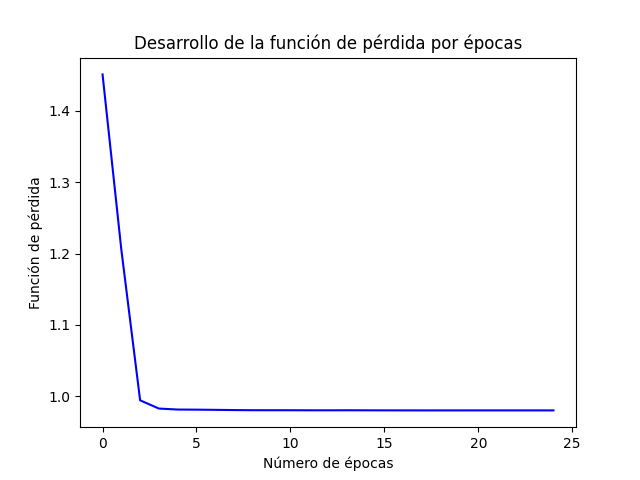
\includegraphics[scale=0.75]{imagenes/loss_autoencoder_fully_connected.png}
	\caption{Evolución de la función de pérdida para el Autoencoder totalmente conectado.}
	\label{img:loss-autoencoder-fully-connected}
\end{figure}

Como podemos ver el valor de la función de pérdida empieza cercano a $1.5$ y consigue descender alrededor de $0.9$. El comportamiento del modelo es como el que queremos ver, empezamos con un valor alto de la función de pérdida y se observa una reducción de su valor. Tras esta reducción considerable podemos ver una estabilización de la misma cuando seguimos aumentando el número de épocas, por lo que podemos deducir que el número de épocas de entrenamiento es suficiente.

El siguiente modelo es el Autoencoder totalmente conectado por lotes. Podemos ver su gráfica en la figura \ref{img:loss-autoencoder-fully-connected-batch}.
\begin{figure}[]
	\centering
	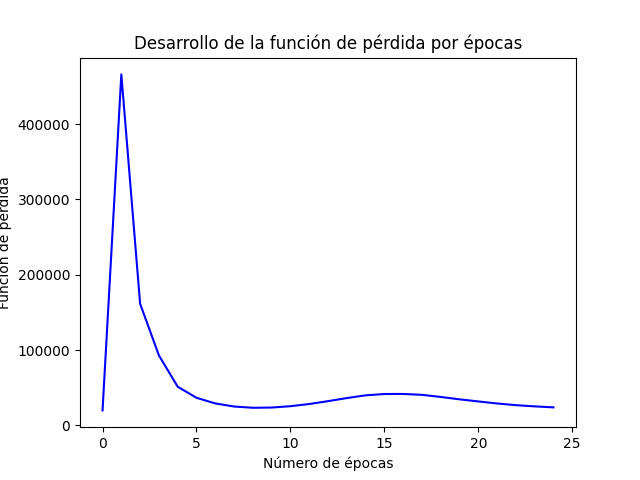
\includegraphics[scale=0.75]{imagenes/loss_autoencoder_fully_connected_batch.png}
	\caption{Evolución de la función de pérdida para el Autoencoder totalmente conectado por lotes.}
	\label{img:loss-autoencoder-fully-connected-batch}
\end{figure}

En este caso podemos ver un comportamiento irregular. En primer lugar podemos ver cómo la primera época (por la inicialización aleatoria de pesos) obtiene una buena loss, luego sube su valor y empieza un descenso suavizado estabilizándose al final. Lo extraño de este comportamiento es que no se estabiliza completamente, ya que tenemos una pequeña crecida y luego una bajada. Además lo peor de todo lo que podemos observar es el valor tan alto de loss que tenemos. Tenemos un valor enorme de la función de pérdida, posiblemente debido a que no estamos consiguiendo que la red aprenda lo suficiente, ya que esto implica que el error acumulado en la reconstrucción de toda la secuencia es muy alto. Se ha probado con secuencias más bajas de tamaño y es claro que el error se reduce hasta bajar a una única instancia, imitando por tanto el comportamiento del modelo anterior. Esto nos puede indicar que este modelo no será muy efectivo en la detección de eventos anómalos, lo veremos en siguientes secciones.

Podemos ver ahora el aprendizaje del Autoencoder con capas LSTM en la figura \ref{img:loss-autoencoder-lstm}.
\begin{figure}[]
	\centering
	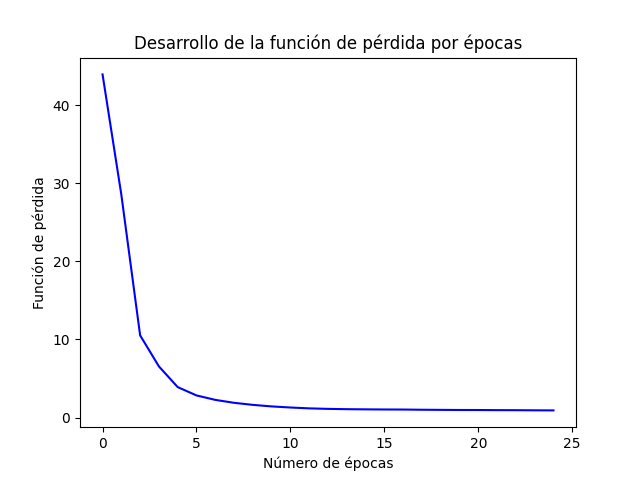
\includegraphics[scale=0.75]{imagenes/loss_autoencoder_lstm.png}
	\caption{Evolución de la función de pérdida para el Autoencoder LSTM.}
	\label{img:loss-autoencoder-lstm}
\end{figure}

De nuevo en este modelo podemos ver un comportamiento adecuado al que buscamos. Empezamos con un valor de la función de pérdida mayor que 40, acabando en un valor cercano a $0.9$ de nuevo. Podemos ver que la progresión en las 5 primeras épocas es muy notoria, reduciéndose el valor de la función de pérdida por debajo de 5. Tras esto se va teniendo una pendiente menos pronunciada hasta que vemos como al final se estabiliza la reducción de la loss. Este comportamiento nos está diciendo que el modelo es capaz de aprender y que además el número de épocas empleadas en el aprendizaje es adecuado.

Podemos ver la gráfica del aprendizaje del modelo de predicción CNN-LSTM en la figura \ref{img:loss-cnn-lstm-forecaster}.
\begin{figure}[]
	\centering
	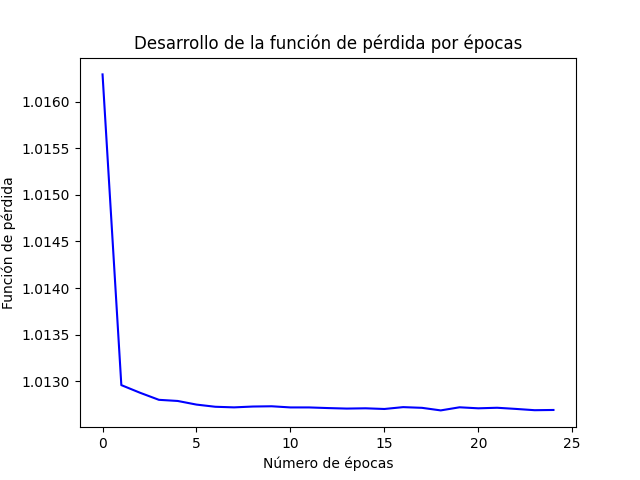
\includegraphics[scale=0.75]{imagenes/loss_cnn_lstm_forecaster.png}
	\caption{Evolución de la función de pérdida para el predictor CNN-LSTM.}
	\label{img:loss-cnn-lstm-forecaster}
\end{figure}

Podemos ver en este caso que los valores de la función de pérdida empiezan bajos, aún así continúan reduciéndose y se estabilizan al final. Con esta gráfica podemos ver que el aprendizaje del modelo es adecuado, ya que consigue una buena loss y se estabilizan los valores, indicando que el número de épocas es suficiente. El valor final de la función de pérdida queda finalmente alrededor de 1.

Por último vemos el aprendizaje del modelo de predicción LSTM en la figura \ref{img:loss-lstm-forecaster}.
\begin{figure}[]
	\centering
	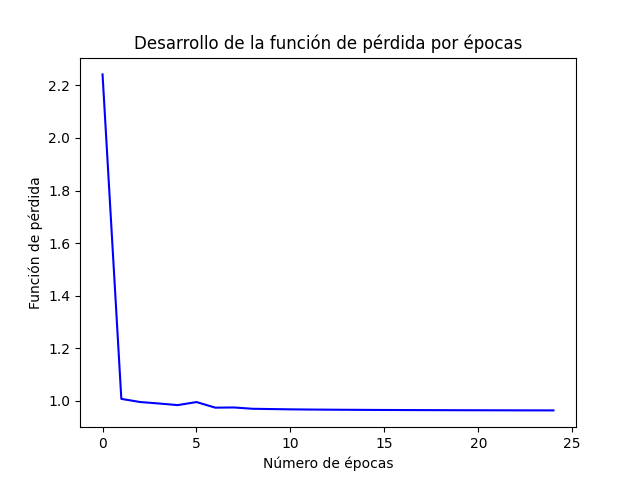
\includegraphics[scale=0.75]{imagenes/loss_lstm_forecasting.png}
	\caption{Evolución de la función de pérdida para el predictor LSTM.}
	\label{img:loss-lstm-forecaster}
\end{figure}

Como podemos ver en este caso también, tenemos un buen aprendizaje del modelo, pues podemos observar una reducción del valor de la función de pérdida desde más de $2.2$ hasta algo maś de $0.9$. Además, podemos ver una reducción muy fuerte de la loss en las primeras etapas y cómo después se estabiliza y se produce muy poca reducción o ninguna. Todo esto nos dice que el modelo ha sido capaz de aprender y además, que el número de épocas empleadas es suficiente para llegar al límite de aprendizaje del modelo o acercarnos al mismo.

Lo siguiente que vamos a hacer es analizar los resultados obtenidos por los modelos con la intención de evaluar la calidad de los mismos y poder discernir el que mejor se comporta de todos ellos.

\section{Resultados obtenidos}

Lo primero que vamos a hacer es ver los resultados de verdaderos positivos, falsos positivos y mantenimientos detectados. En el periodo de prueba que hemos escogido tenemos 28 mantenimientos totales que podemos detectar. Es claro que nos interesa detectar cuantos más mantenimientos mejor, pero si tenemos un modelo que a cambio nos da muchos falsos positivos no es una buena elección. Por poner un ejemplo evidente, si tenemos un modelo que siempre da alerta entonces va a detectar todos los mantenimientos, pero también va a tener un número muy elevado de falsos positivos.

Por ello el mejor modelo no podemos elegirlo sólo en base al número de mantenimientos que detectamos sobre el total, tendremos que sopesar también el resto de métricas. Por tanto veamos ahora la tabla de resultados:

\begin{table}[H]
	\centering
	\begin{tabular}{|l|c|c|c|c|}
		\hline
		\multicolumn{1}{|c|}{\textbf{Modelo}} & \textbf{TP} & \textbf{FP} & \textbf{Mant. Detectados} & \textbf{Mant. Totales} \\ \hline
		\textbf{AE FCC}                       & 33          & 441         & 20                                 & 28                              \\ \hline
		\textbf{AE FCC lotes}                 & 33          & 393         & 20                                 & 28                              \\ \hline
		\textbf{AE LSTM}                      & 33          & 447         & 20                                 & 28                              \\ \hline
		\textbf{Predictor LSTM}               & 33          & 393         & 20                                 & 28                              \\ \hline
		\textbf{Predictor CNN-LSTM}           & 35          & 213         & 22                                 & 28                              \\ \hline
		\textbf{FB LOF}                       & 15          & \textbf{56} & 8                                  & 28                              \\ \hline
		\textbf{HBOS}                         & \textbf{44} & 505         & \textbf{23}                        & 28                              \\ \hline
		\textbf{IForest}                      & 28          & 344         & 19                                 & 28                              \\ \hline
		\textbf{KNN}                          & 42          & 505         & \textbf{23}                        & 28                              \\ \hline
		\textbf{LODA}                         & 36          & 341         & 22                                 & 28                              \\ \hline
		\textbf{LOF}                          & 40          & 471         & 22                                 & 28                              \\ \hline
		\textbf{PCA}                          & 26          & 256         & 16                                 & 28                              \\ \hline
	\end{tabular}
	\caption{Tabla de resultados generales de los modelos a comparar.}
	\label{tabla:resultados1}
\end{table}

La primera métrica que tenemos que observar en esta tabla es la de mantenimientos detectados. Podemos ver que en total tenemos 28 mantenimientos y tenemos dos métodos con 23 mantenimientos detectados y tres con 22 mantenimientos detectados. Entre estos, si no tuviéramos más información, lo lógico es decir que los mejores modelos son aquellos que más mantenimientos detectan. Sabiendo lo que hemos discutido anteriormente esto no es así, ya que debemos intentar también maximizar los verdaderos positivos (cuantos más verdaderos positivos tengamos más certeza tenemos de la detección de los mantenimientos) y minimizar los falsos positivos.

A la vista está que todos los modelos tienen un alto número de falsos positivos, pero vamos a intentar ver cuáles tienen mejores números entre los considerados. Por supuesto la intención es maximizar los verdaderos positivos y minimizar los falsos positivos. Los dos modelos que más mantenimientos predicen correctamente podemos ver que tienen 505 falsos positivos ambos. Esto es una cifra altísima, que nos está indicando que casi siempre dan alerta y por tanto aciertan más mantenimientos a costa de fallar mucho más en las zonas normales. Por contra, podemos ver que LOF y LODA cometen algunos menos falsos positivos sólo fallando un mantenimiento más, pero el mejor de todos en este sentido es el predictor CNN-LSTM que baja los falsos positivos a 213, menos de la mitad de los que cometen HBOS y KNN sólo por un mantenimiento más.

Es por esto que, con estas métricas, podemos decir que el modelo de predicción CNN-LSTM se comporta mejor que el resto ya que consigue predecir 22 de los 28 mantenimientos con 35 verdaderos positivos y sólo 213 falsos positivos. En la métrica de los falsos positivos es el que menos fallos comete después del modelo Feature Bagging LOF, que sólo tiene 56 falsos positivos pero predice correctamente únicamente 8 mantenimientos de los 28. 

Este problema no es un problema de clasificación al uso, aunque podemos intentar convertirlo en un problema de clasificación de dos clases. Cuando damos alerta y hay un mantenimiento cerca tenemos un verdadero positivo, cuando tenemos un mantenimiento cerca pero no damos alerta tenemos un falso negativo, cuando no tenemos mantenimiento cerca y damos la alerta tenemos un falso positivo y si no tenemos un mantenimiento cerca y no damos la alerta entonces tenemos un verdadero negativo. Con esta distribución podemos sacar la matriz de confusión clásica de un problema de dos clases con TP, TN, FP y FN, por lo que podemos sacar algunas métricas más.

\begin{table}[H]
	\centering
	\begin{tabular}{|l|c|c|c|c|}
		\hline
		\multicolumn{1}{|c|}{\textbf{Modelo}} & \textbf{TP} & \textbf{FP} & \textbf{TN}  & \textbf{FN} \\ \hline
		\textbf{AE FCC}                       & 33          & 441         & 75           & 8           \\ \hline
		\textbf{AE FCC lotes}                 & 33          & 393         & 123          & 8           \\ \hline
		\textbf{AE LSTM}                      & 33          & 447         & 69           & 8           \\ \hline
		\textbf{Predictor LSTM}               & 33          & 393         & 123          & 8           \\ \hline
		\textbf{Predictor CNN-LSTM}           & 35          & 213         & 301          & 8           \\ \hline
		\textbf{FB LOF}                       & 15          & \textbf{56} & \textbf{340} & 20          \\ \hline
		\textbf{HBOS}                         & \textbf{44} & 505         & 0            & \textbf{5}  \\ \hline
		\textbf{IForest}                      & 28          & 344         & 177          & 9           \\ \hline
		\textbf{KNN}                          & 42          & 505         & 1            & \textbf{5}  \\ \hline
		\textbf{LODA}                         & 36          & 341         & 172          & 6           \\ \hline
		\textbf{LOF}                          & 40          & 471         & 38           & 6           \\ \hline
		\textbf{PCA}                          & 26          & 256         & 267          & 12          \\ \hline
	\end{tabular}
	\caption{Tabla con los verdaderos positivos, falsos positivos, verdaderos negativos y falsos negativos.}
	\label{tabla:resultados2}
\end{table}

Estamos ante un problema de clasificación con dos clases muy desbalanceado, como podemos suponer. Está claro que vamos a tener un número mucho mayor de zonas sin alerta real (no están cerca de un mantenimiento) que zonas en las que deberíamos de dar la alerta. Además, también está claro que es más valioso para la empresa detectar las alertas que las zonas normales ya que las alertas implican la parada de la maquinaria y por tanto una pérdida de tiempo de trabajo y dinero.

Teniendo esto claro, la tabla \ref{tabla:resultados2} nos refleja el desempeño de los modelos al intentar predecir las alertas de mantenimiento y las zonas normales. Lo que vamos a querer es maximizar los verdaderos positivos y verdaderos negativos e intentar minimizar los falsos positivos y falsos negativos.

Como podemos observar en la tabla, el modelo que menos falsos positivos comete y más verdaderos negativos tiene es Feature Bagging LOF. En la tabla anterior comentamos el posible comportamiento de este modelo, pero ahora lo podemos tener algo más claro. El modelo no da la alerta casi nunca y por tanto predice correctamente muy pocos mantenimientos, por contra al no dar muchas alarmas, es capaz de detectar correctamente muchos periodos normales. Este comportamiento no nos es nada útil pues estamos primando la detección de la normalidad frente a las anomalías.

Por otro lado, podemos ver que el modelo que más verdaderos positivos da es HBOS con 44. Además este modelo es el que menos falsos negativos nos produce junto con el modelo KNN. Lo interesante de esta tabla es que, si quitamos el modelo Feature Bagging LOF de la ecuación, el predictor CNN-LSTM es el que más verdaderos negativos tiene y el que menos falsos positivos tiene entre todos los modelos considerados. Esto junto con el hecho de que no tiene muchos menos verdaderos positivos que HBOS ni muchos más falsos negativos hace que sea un modelo más equilibrado.

En este problema tenemos dos formas de calcular el acierto de los modelos: podemos calcular el porcentaje de mantenimientos detectados y podemos calcular el acierto de verdaderos positivos y verdaderos negativos sobre el total. La segunda de las formas lo que pretende es que, el modelo con acierto perfecto debería de ser capaz de dar alarma en todas las ventanas temporales que caigan 6 horas antes de un mantenimiento y debería ser capaz de no dar ninguna alarma en el resto de ventanas temporales. Por tanto estaríamos calculando el porcentaje de acierto sobre las ventanas temporales y no sobre los mantenimientos directamente.

\begin{table}[H]
	\centering
	\begin{tabular}{|l|c|c|}
		\hline
		\multicolumn{1}{|c|}{\textbf{Modelo}} & \textbf{\begin{tabular}[c]{@{}c@{}}Tasa mantenimientos\\ detectados\end{tabular}} & \textbf{\begin{tabular}[c]{@{}c@{}}Acierto sobre\\ ventanas\end{tabular}} \\ \hline
		\textbf{AE FCC}                       & 0.7143                                                                            & 0.1939                                                                    \\ \hline
		\textbf{AE FCC lotes}                 & 0.7143                                                                            & 0.2801                                                                    \\ \hline
		\textbf{AE LSTM}                      & 0.7143                                                                            & 0.1831                                                                    \\ \hline
		\textbf{Predictor LSTM}               & 0.7143                                                                            & 0.2801                                                                    \\ \hline
		\textbf{Predictor CNN-LSTM}           & 0.7857                                                                            & 0.6054                                                                    \\ \hline
		\textbf{FB LOF}                       & 0.2857                                                                            & \textbf{0.8237}                                                           \\ \hline
		\textbf{HBOS}                         & \textbf{0.8214}                                                                   & 0.0794                                                                    \\ \hline
		\textbf{IForest}                      & 0.6786                                                                            & 0.3674                                                                    \\ \hline
		\textbf{KNN}                          & \textbf{0.8214}                                                                   & 0.0794                                                                    \\ \hline
		\textbf{LODA}                         & 0.7857                                                                            & 0.3748                                                                    \\ \hline
		\textbf{LOF}                          & 0.7857                                                                            & 0.1405                                                                    \\ \hline
		\textbf{PCA}                          & 0.5714                                                                            & 0.5223                                                                    \\ \hline
	\end{tabular}
	\caption{Tabla con los aciertos de los modelos.}
	\label{tabla:resultados3}
\end{table}

En la columna de tasa de mantenimientos detectados vemos que no tenemos ninguna sorpresa, ya que lo hemos analizado previamente cuando hemos visto el número de mantenimientos que detectaba cada uno de los modelos. En la columna de acierto sobre ventanas tenemos alguna sorpresa más. Como podemos ver el modelo que mejor resultado da es Feature Bagging LOF, lo cual es razonable. Ya hemos comentado que hay muchas más ventanas en zonas de normalidad que en zonas anómalas, por lo que el modelo, al no dar casi alarmas, acierta casi todas las ventanas. Si eliminamos este modelo de la ecuación podemos ver que el siguiente mejor modelo es el predictor CNN-LSTM. Esta tabla nos está diciendo que deberíamos emplear alguna métrica de problemas de clasificación desbalanceada para poder comparar mejor los aciertos, por tanto vamos a ver la tasa de positivos y negativos y vamos a utilizar la multiplicación de las mismas como métrica.

\begin{table}[H]
	\centering
	\begin{tabular}{|l|c|c|l|}
		\hline
		\multicolumn{1}{|c|}{\textbf{Modelo}} & \textbf{TPR}    & \textbf{TNR}    & \multicolumn{1}{c|}{\textbf{TPRxTNR}} \\ \hline
		\textbf{AE FCC}                       & 0.8049          & 0.1453          & 0.1170                                \\ \hline
		\textbf{AE FCC lotes}                 & 0.8049          & 0.2384          & 0.1919                                \\ \hline
		\textbf{AE LSTM}                      & 0.8049          & 0.1337          & 0.1076                                \\ \hline
		\textbf{Predictor LSTM}               & 0.8049          & 0.2384          & 0.1919                                \\ \hline
		\textbf{Predictor CNN-LSTM}           & 0.8537          & 0.5856          & \textbf{0.5}                          \\ \hline
		\textbf{FB LOF}                       & 0.4286          & \textbf{0.8586} & 0.3680                                \\ \hline
		\textbf{HBOS}                         & \textbf{0.8980} & 0               & 0                                     \\ \hline
		\textbf{IForest}                      & 0.7568          & 0.3397          & 0.2571                                \\ \hline
		\textbf{KNN}                          & 0.8959          & 0.0020          & 0.0018                                \\ \hline
		\textbf{LODA}                         & 0.8571          & 0.3353          & 0.2874                                \\ \hline
		\textbf{LOF}                          & 0.8696          & 0.0747          & 0.0649                                \\ \hline
		\textbf{PCA}                          & 0.6842          & 0.5105          & 0.3493                                \\ \hline
	\end{tabular}
	\caption{Tabla con las tasas de positivos y negativos.}
	\label{tabla:resultados4}
\end{table}

En esta tabla podemos ver la tasa de acierto de positivos, la de negativos y la multiplicación de ambas. La intención de multiplicar ambas tasas es que podemos tener una buena puntuación en alguna de ellas pero muy mala en la otra. Esto nos estaría diciendo que nuestro modelo está desequilibrado y por tanto predice mejor los positivos o los negativos únicamente. 

Esto se puede ver claramente. Parecía que el mejor modelo hasta ahora podía ser HBOS pero podemos ver que la tasa de acierto de negativos es 0, por lo que el modelo está altamente desbalanceado y la tasa al multiplicar sale cero. Por otro lado Feature Bagging LOF podemos ver que acierta muchos negativos, pero falla muchos positivos que son los más importantes. En el caso de KNN y LOF podemos ver que tienen muy buenas tasas de acierto de positivos pero pésimas tasas de acierto de negativos y finalmente podemos ver que LODA tiene algo más de equilibrio, pero el mejor modelo ahora es el predictor CNN-LSTM que es el que mejor puntuación saca al multiplicar las dos tasas de acierto. Esto nos está diciendo que es el más equilibrado de todos con una tasa de acierto en los positivos de un $85.37\%$ y en negativos de un $58.56\%$.

\begin{table}[H]
	\centering
	\begin{tabular}{|l|c|c|}
		\hline
		\multicolumn{1}{|c|}{\textbf{Modelo}} & \textbf{F1}     & \textbf{AUC}  \\ \hline
		\textbf{AE FCC}                       & 0.1282          & 0.48          \\ \hline
		\textbf{AE FCC lotes}                 & 0.1413          & 0.52          \\ \hline
		\textbf{AE LSTM}                      & 0.1267          & 0.47          \\ \hline
		\textbf{Predictor LSTM}               & 0.1413          & 0.52          \\ \hline
		\textbf{Predictor CNN-LSTM}           & 0.2422          & \textbf{0.72} \\ \hline
		\textbf{FB LOF}                       & \textbf{0.2830} & 0.64          \\ \hline
		\textbf{HBOS}                         & 0.1471          & 0.45          \\ \hline
		\textbf{IForest}                      & 0.1369          & 0.55          \\ \hline
		\textbf{KNN}                          & 0.1443          & 0.45          \\ \hline
		\textbf{LODA}                         & 0.1718          & 0.6           \\ \hline
		\textbf{LOF}                          & 0.1436          & 0.47          \\ \hline
		\textbf{PCA}                          & 0.1625          & 0.6           \\ \hline
	\end{tabular}
	\caption{Tabla de resultados con F1 y AUC.}
	\label{tabla:resultados5}
\end{table}

La medida F1 nos mide el número de verdaderos positivos que tenemos en relación a la media de falsos positivos y falsos negativos, por lo que cuanto más alto sea el valor y más cercano a 1 mejor será el modelo. En este caso tenemos claro que cometemos muchos falsos positivos, por lo que los modelos sufren una penalización muy grande en esta métrica. Podemos ver que Feature Bagging LOF es el que mejores números obtiene en esta métrica, pero ya sabemos que no es comparable. El siguiente modelo es el predictor CNN-LSTM, por lo que podemos decir que este modelo es el mejor en esta métrica. 

En la siguiente columna tenemos el AUC o Área Bajo la Curva ROC en este caso. La curva ROC es una curva en la que contraponemos en el eje X la tasa de falsos positivos y en el eje Y la tasa de verdaderos positivos variando el umbral probabilístico en el que consideramos que tenemos un positivo o un negativo. En este caso no podemos variar este umbral, por lo que sólo vamos a tener un punto. A mayor área bajo esta curva mejor y cuanto más cercano sea el punto de la curva al $(1,0)$ mejor. Por tanto en el mejor de los casos la curva ROC será la parte superior de un cuadrado y el AUC 1, mientras que en el peor de los casos también tendremos AUC 1 pero tendremos ahora la curva ROC el lado inferior del cuadrado. Veamos por tanto las gráficas ROC:

\begin{figure}[H]
	\centering
	\begin{subfigure}{.49\textwidth}
		\centering
		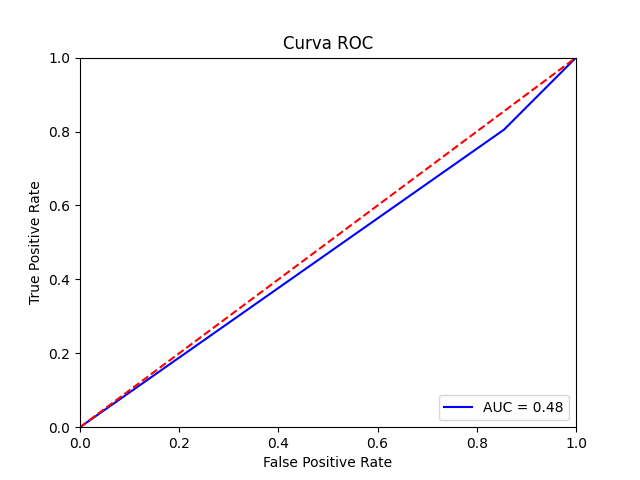
\includegraphics[scale=0.42]{imagenes/roc/Autoencoder-Fully-Connected_roc.png}
		\caption{Autoencoder totalmente conectado.}
	\end{subfigure}
	\begin{subfigure}{.49\textwidth}
		\centering
		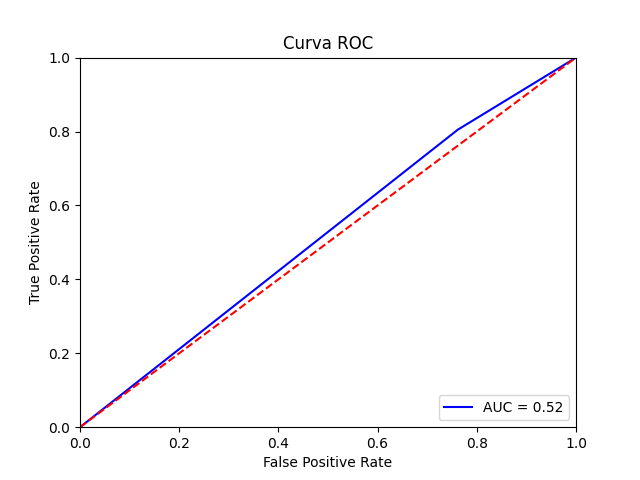
\includegraphics[scale=0.42]{imagenes/roc/Autoencoder-Fully-Connected-Lotes_roc.png}
		\caption{Autoencoder totalmente conectado por lotes.}
	\end{subfigure}
	\label{img:roc1}
\end{figure}

\begin{figure}[H]
	\centering
	\begin{subfigure}{.49\textwidth}
		\centering
		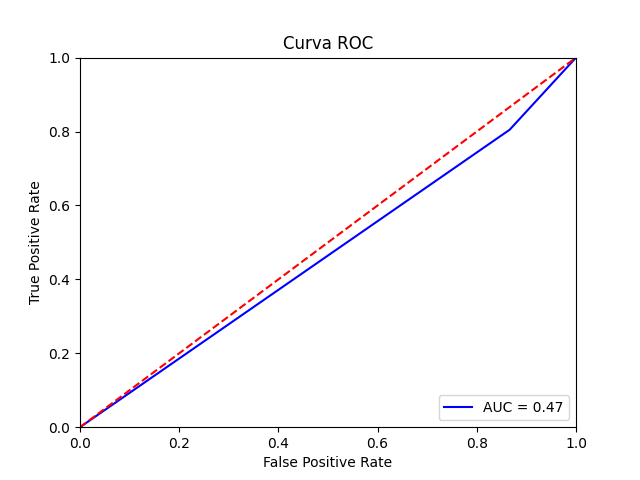
\includegraphics[scale=0.42]{imagenes/roc/Autoencoder-LSTM_roc.png}
		\caption{Autoencoder LSTM.}
	\end{subfigure}
	\begin{subfigure}{.49\textwidth}
		\centering
		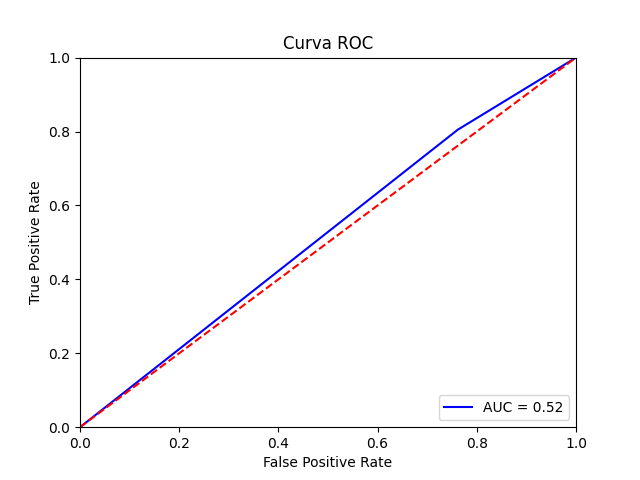
\includegraphics[scale=0.42]{imagenes/roc/Predictor-LSTM_roc.png}
		\caption{Modelo de predicción LSTM.}
	\end{subfigure}
	\label{img:roc2}
\end{figure}

\begin{figure}[H]
	\centering
	\begin{subfigure}{.49\textwidth}
		\centering
		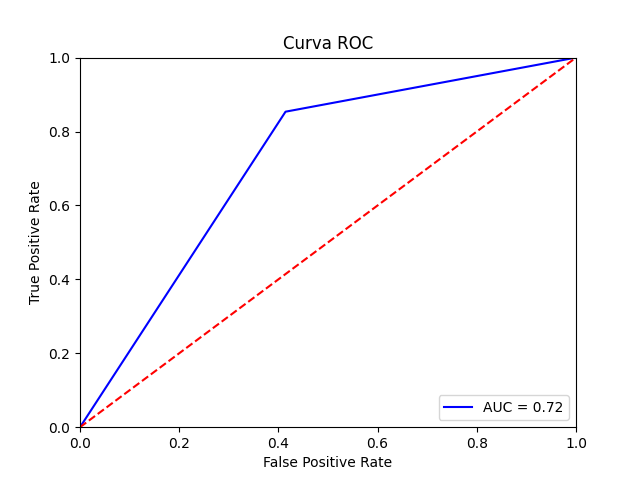
\includegraphics[scale=0.42]{imagenes/roc/Predictor-CNN-LSTM_roc.png}
		\caption{Predictor CNN-LSTM.}
	\end{subfigure}
	\begin{subfigure}{.49\textwidth}
		\centering
		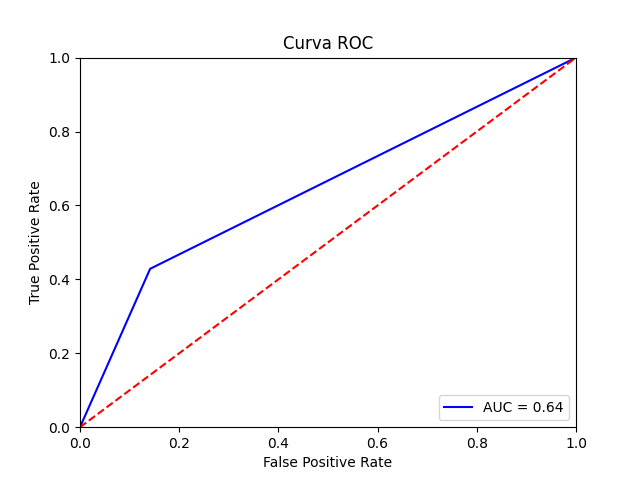
\includegraphics[scale=0.42]{imagenes/roc/Feature-Bagging-LOF_roc.png}
		\caption{Feature Bagging LOF.}
	\end{subfigure}
	\label{img:roc3}
\end{figure}

\begin{figure}[H]
	\centering
	\begin{subfigure}{.49\textwidth}
		\centering
		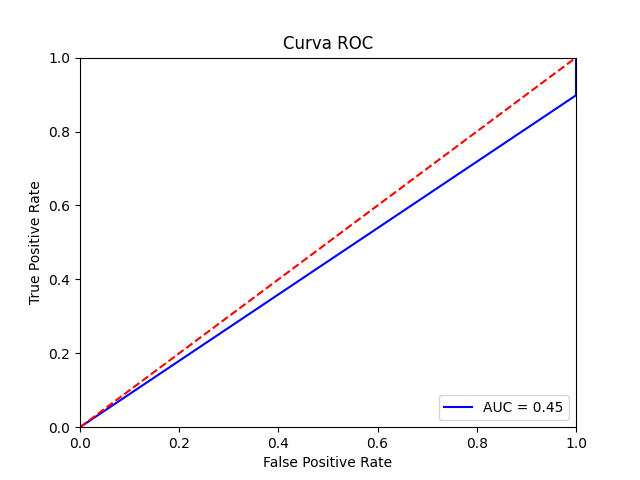
\includegraphics[scale=0.42]{imagenes/roc/HBOS_roc.png}
		\caption{HBOS.}
	\end{subfigure}
	\begin{subfigure}{.49\textwidth}
		\centering
		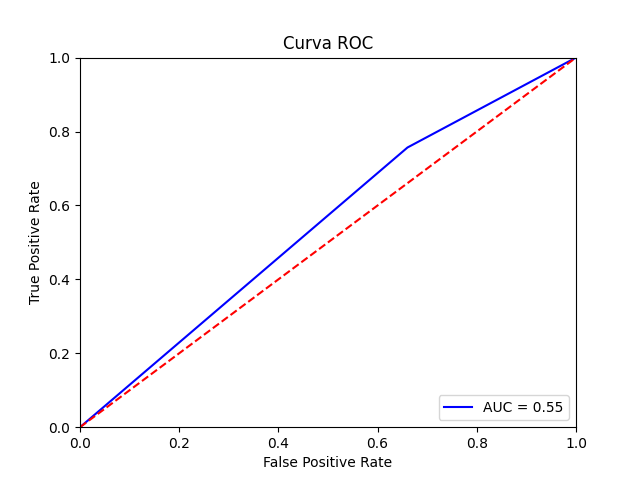
\includegraphics[scale=0.42]{imagenes/roc/Isolation-Forest_roc.png}
		\caption{Isolation Forest.}
	\end{subfigure}
	\label{img:roc4}
\end{figure}

\begin{figure}[H]
	\centering
	\begin{subfigure}{.49\textwidth}
		\centering
		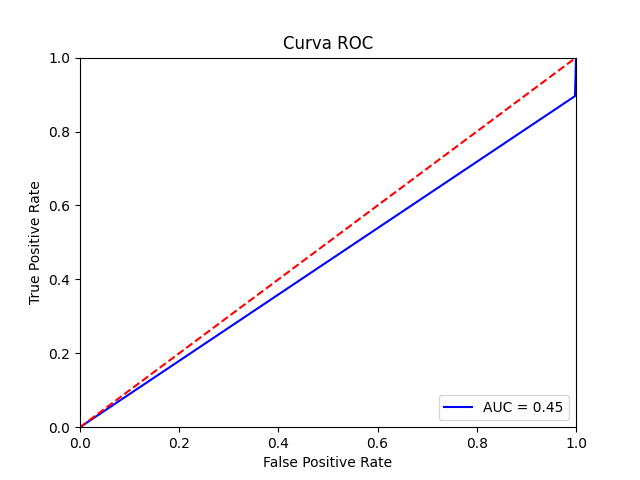
\includegraphics[scale=0.42]{imagenes/roc/KNN_roc.png}
		\caption{KNN.}
	\end{subfigure}
	\begin{subfigure}{.49\textwidth}
		\centering
		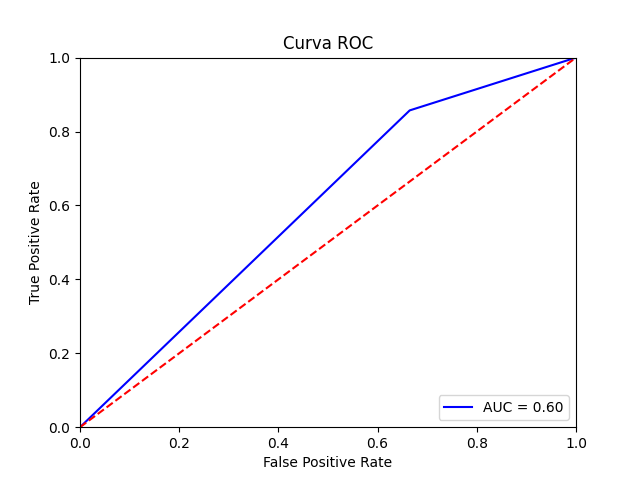
\includegraphics[scale=0.42]{imagenes/roc/LODA_roc.png}
		\caption{LODA.}
	\end{subfigure}
	\label{img:roc5}
\end{figure}

\begin{figure}[H]
	\centering
	\begin{subfigure}{.49\textwidth}
		\centering
		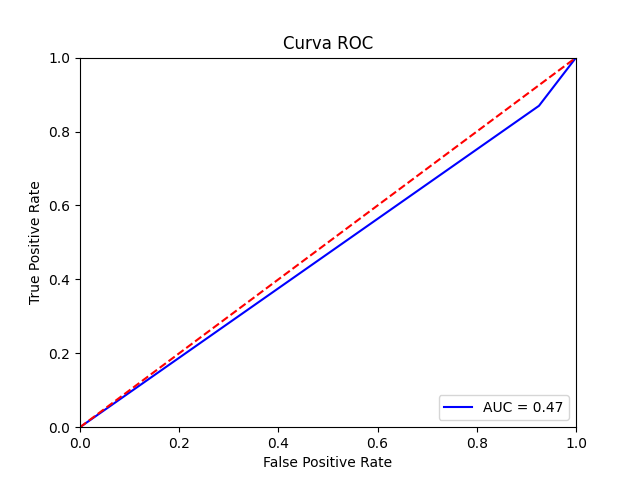
\includegraphics[scale=0.42]{imagenes/roc/LOF_roc.png}
		\caption{LOF.}
	\end{subfigure}
	\begin{subfigure}{.49\textwidth}
		\centering
		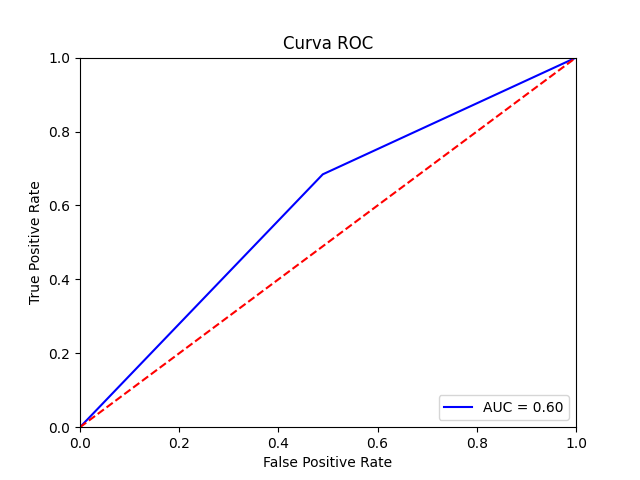
\includegraphics[scale=0.42]{imagenes/roc/PCA_roc.png}
		\caption{PCA.}
	\end{subfigure}
	\label{img:roc6}
\end{figure}

En las gráficas podemos ver que tenemos una línea roja discontinua en medio. Esta línea nos marca el comportamiento de un modelo aleatorio, que tendría la misma efectividad que lanzar una moneda al aire y discernir la clase de forma aleatoria según una uniforme. La intención es que los mejores modelos estén por encima de esta línea y si el modelo está por debajo es que es peor que un modelo aleatorio.

Podemos ver que el mejor de los modelos según la curva ROC es el predictor CNN-LSTM con un AUC de $0.72$. Por contra aquí podemos ver que la tasa de falsos positivos hace que los modelos KNN y HBOS tengan las peores curvas ROC de todas. En cuanto al modelo FeatureBagging LOF hemos visto ya que no acierta lo suficiente como para tenerlo en consideración y podemos ver que PCA tiene un comportamiento razonablemente equilibrado pero sólo predicen correctamente 16 de los 28 mantenimientos por lo que no está a la altura del resto de modelos. Por otro lado tenemos a LODA que tiene un comportamiento razonablemente bueno pero es peor aún así que el predictor CNN-LSTM.

Por tanto de nuevo hemos podido ver que el modelo de predicción CNN-LSTM es el modelo que mejor resultado nos ha arrojado en estas métricas.

Por último vamos a comparar los tiempos de los modelos. Hay que recordar que los modelos clásicos de detección de anomalías no tienen un periodo de entrenamiento pues no hay etiquetas de las que aprender. En cambio en los modelos Deep Learning si que tenemos un periodo de entrenamiento que vamos a comparar ahora entre modelos:

\begin{figure}[H]
	\centering
	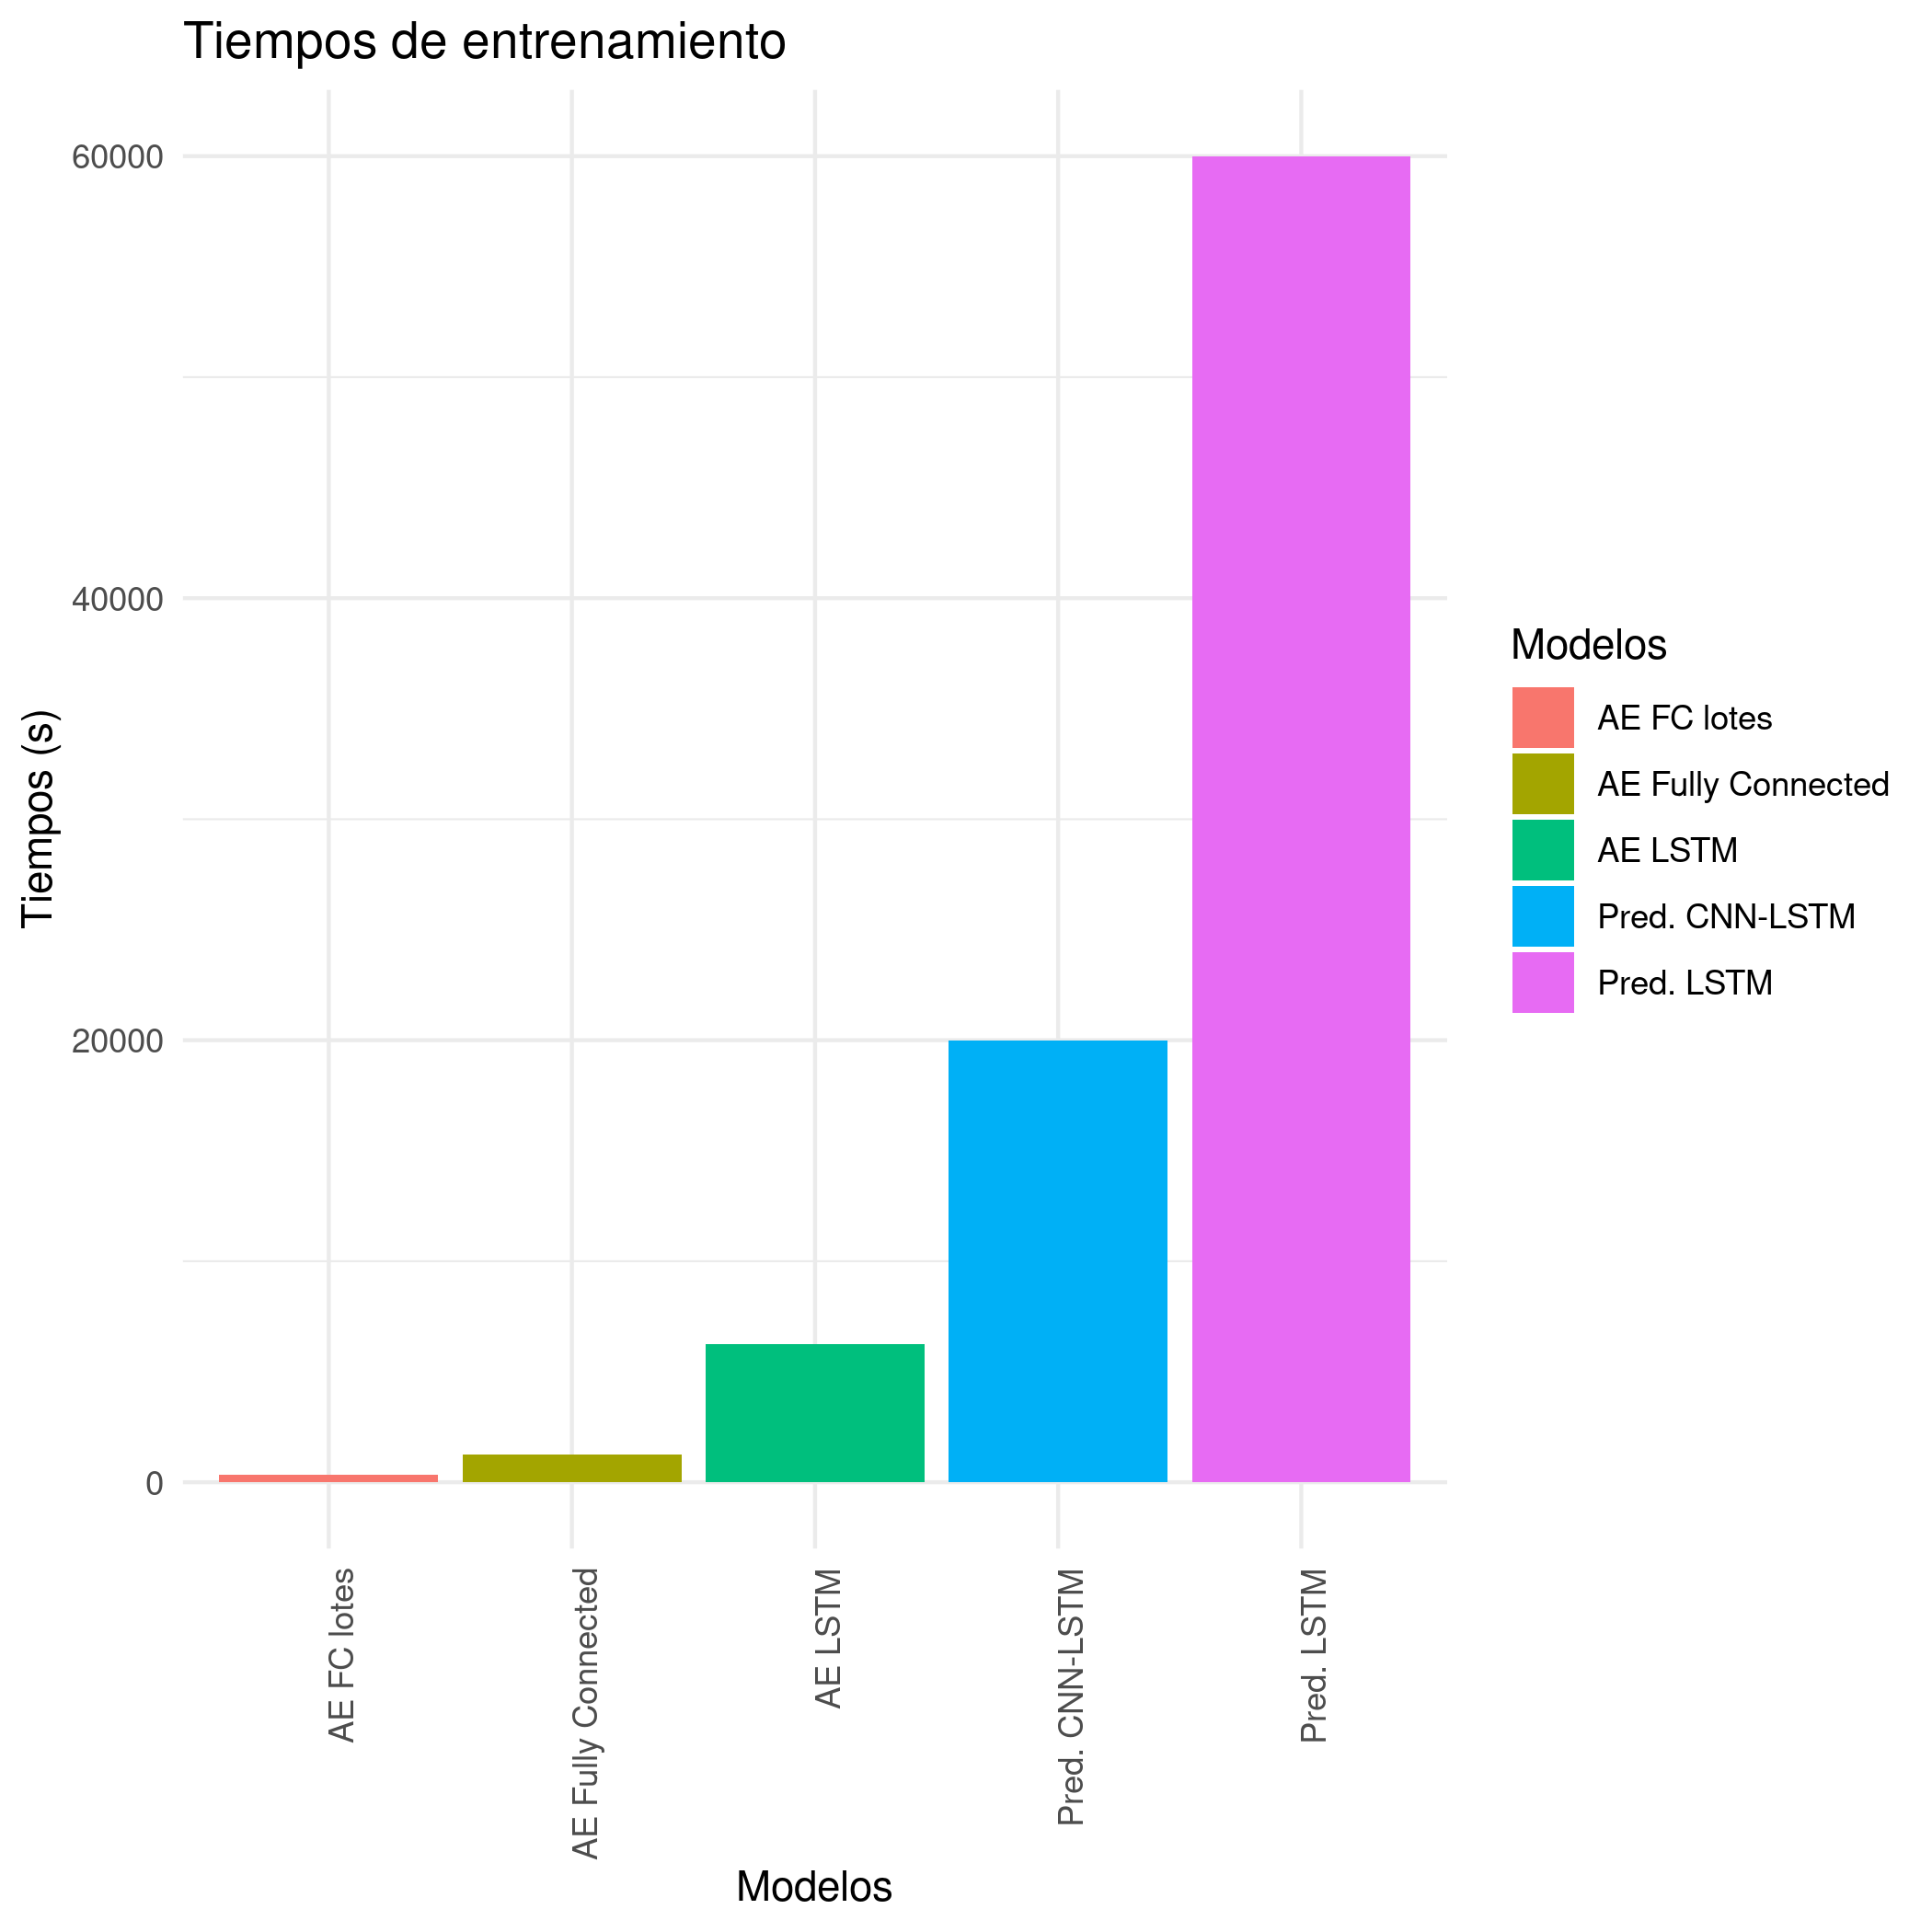
\includegraphics[scale=0.65]{imagenes/tiempos_entrenamiento.png}
	\caption{Tiempos de entrenamiento modelos Deep Learning.}
	\label{img:tiempos-entrenamiento}
\end{figure}

Aquí podemos ver que los modelos tienen tiempos de entrenamiento muy distintos. En primer lugar todos los modelos Autoencoder tienen tiempos de entrenamiento bastante bajos, mientras que los modelos de predicción tienen tiempos de entrenamiento mucho más altos. En particular podemos ver cómo los modelos totalmente conectados son los que menor tiempo de entrenamiento tienen mientras que el que más es el modelo de predicción puramente LSTM.

Este tiempo es importante pero sólo vamos a tener que entrenar por completo un modelo una vez, por lo que lo que más nos interesa es cuánto tardamos en predecir un día completo de datos. Estos tiempos hacen referencia a cuánto tardamos en obtener los scores del modelo, no en el proceso completo. No necesitamos saber cuánto tardamos en el resto del proceso para comparar los modelos, pues las operaciones siempre son las mismas a partir de tener los scores. Los tiempos que varían son los que cada modelo consume para poder sacar las puntuaciones de anomalía, veamos las gráficas por tanto:

\begin{figure}[H]
	\centering
	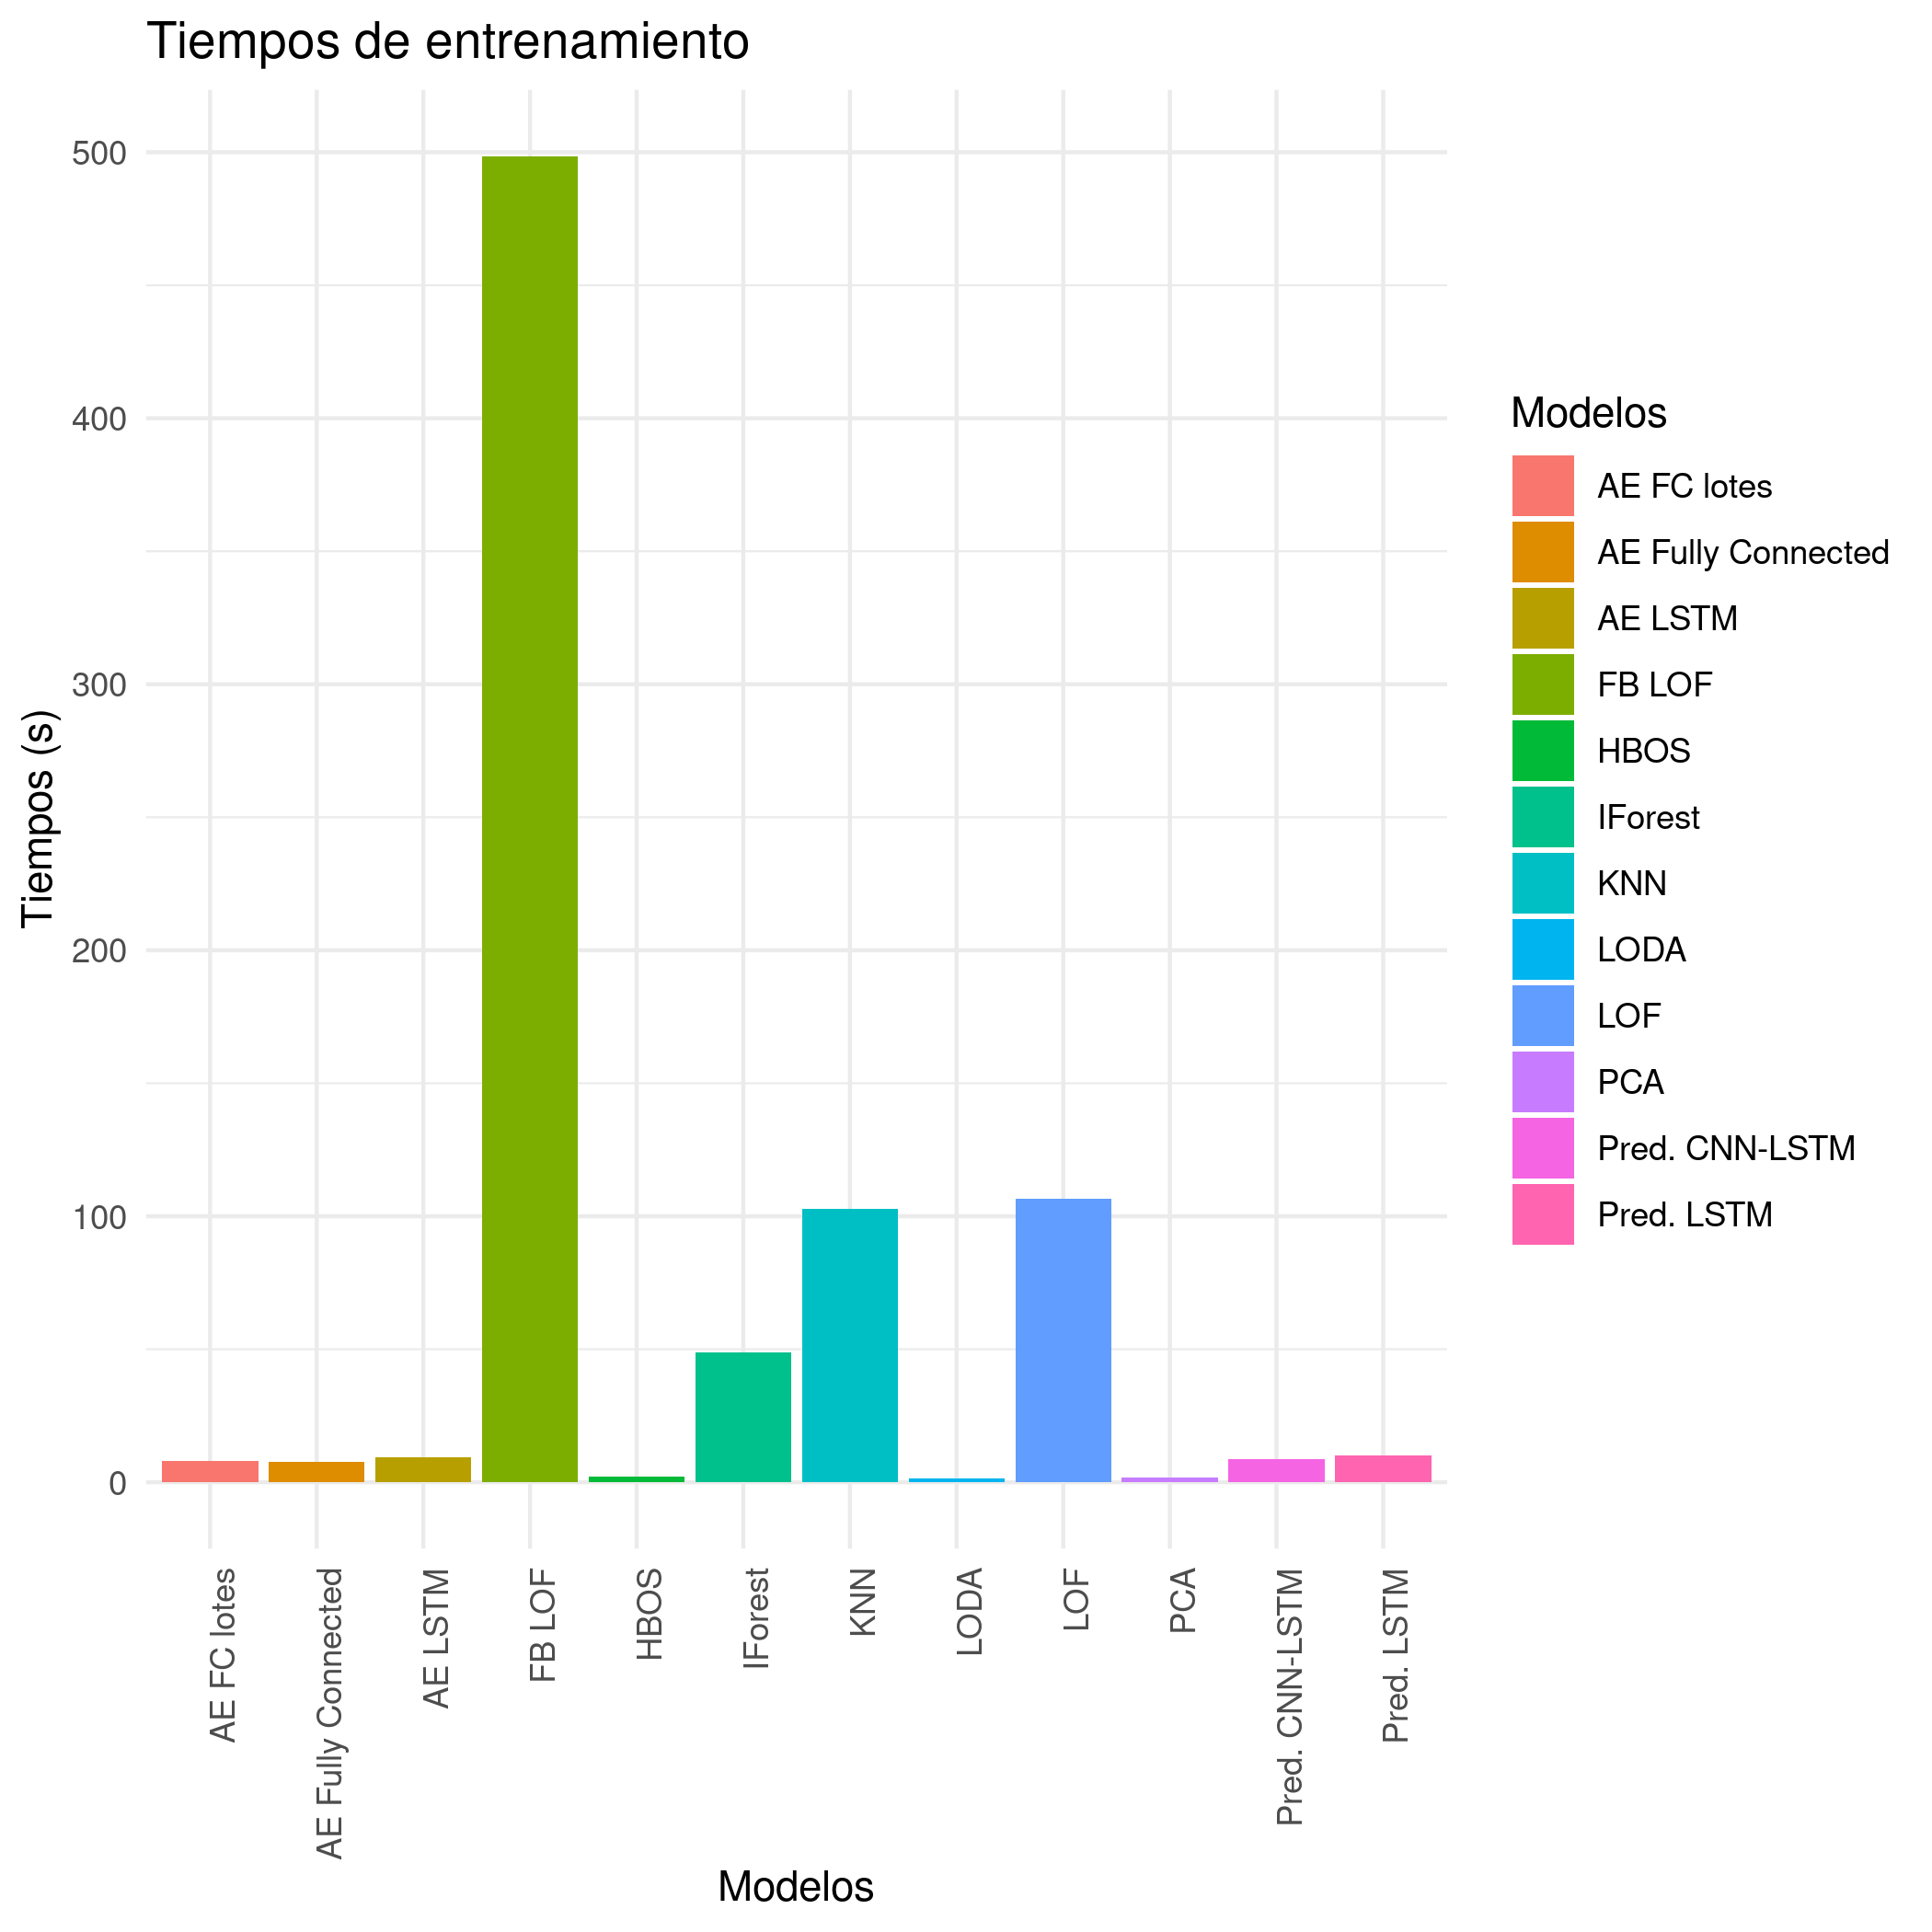
\includegraphics[scale=0.65]{imagenes/tiempos_prediccion.png}
	\caption{Tiempos de predicción de los modelos.}
	\label{img:tiempos-prediccion}
\end{figure}

Podemos ver que el modelo que más tiempo consume (dando malos resultados) es el modelo Feature Bagging LOF que nos está distorsionando un poco la escala de la gráfica. Ya que hemos comprobado que su desempeño en tiempo es malo vamos a eliminarlo de la misma para poder ver mejor el resto de modelos:

\begin{figure}[H]
	\centering
	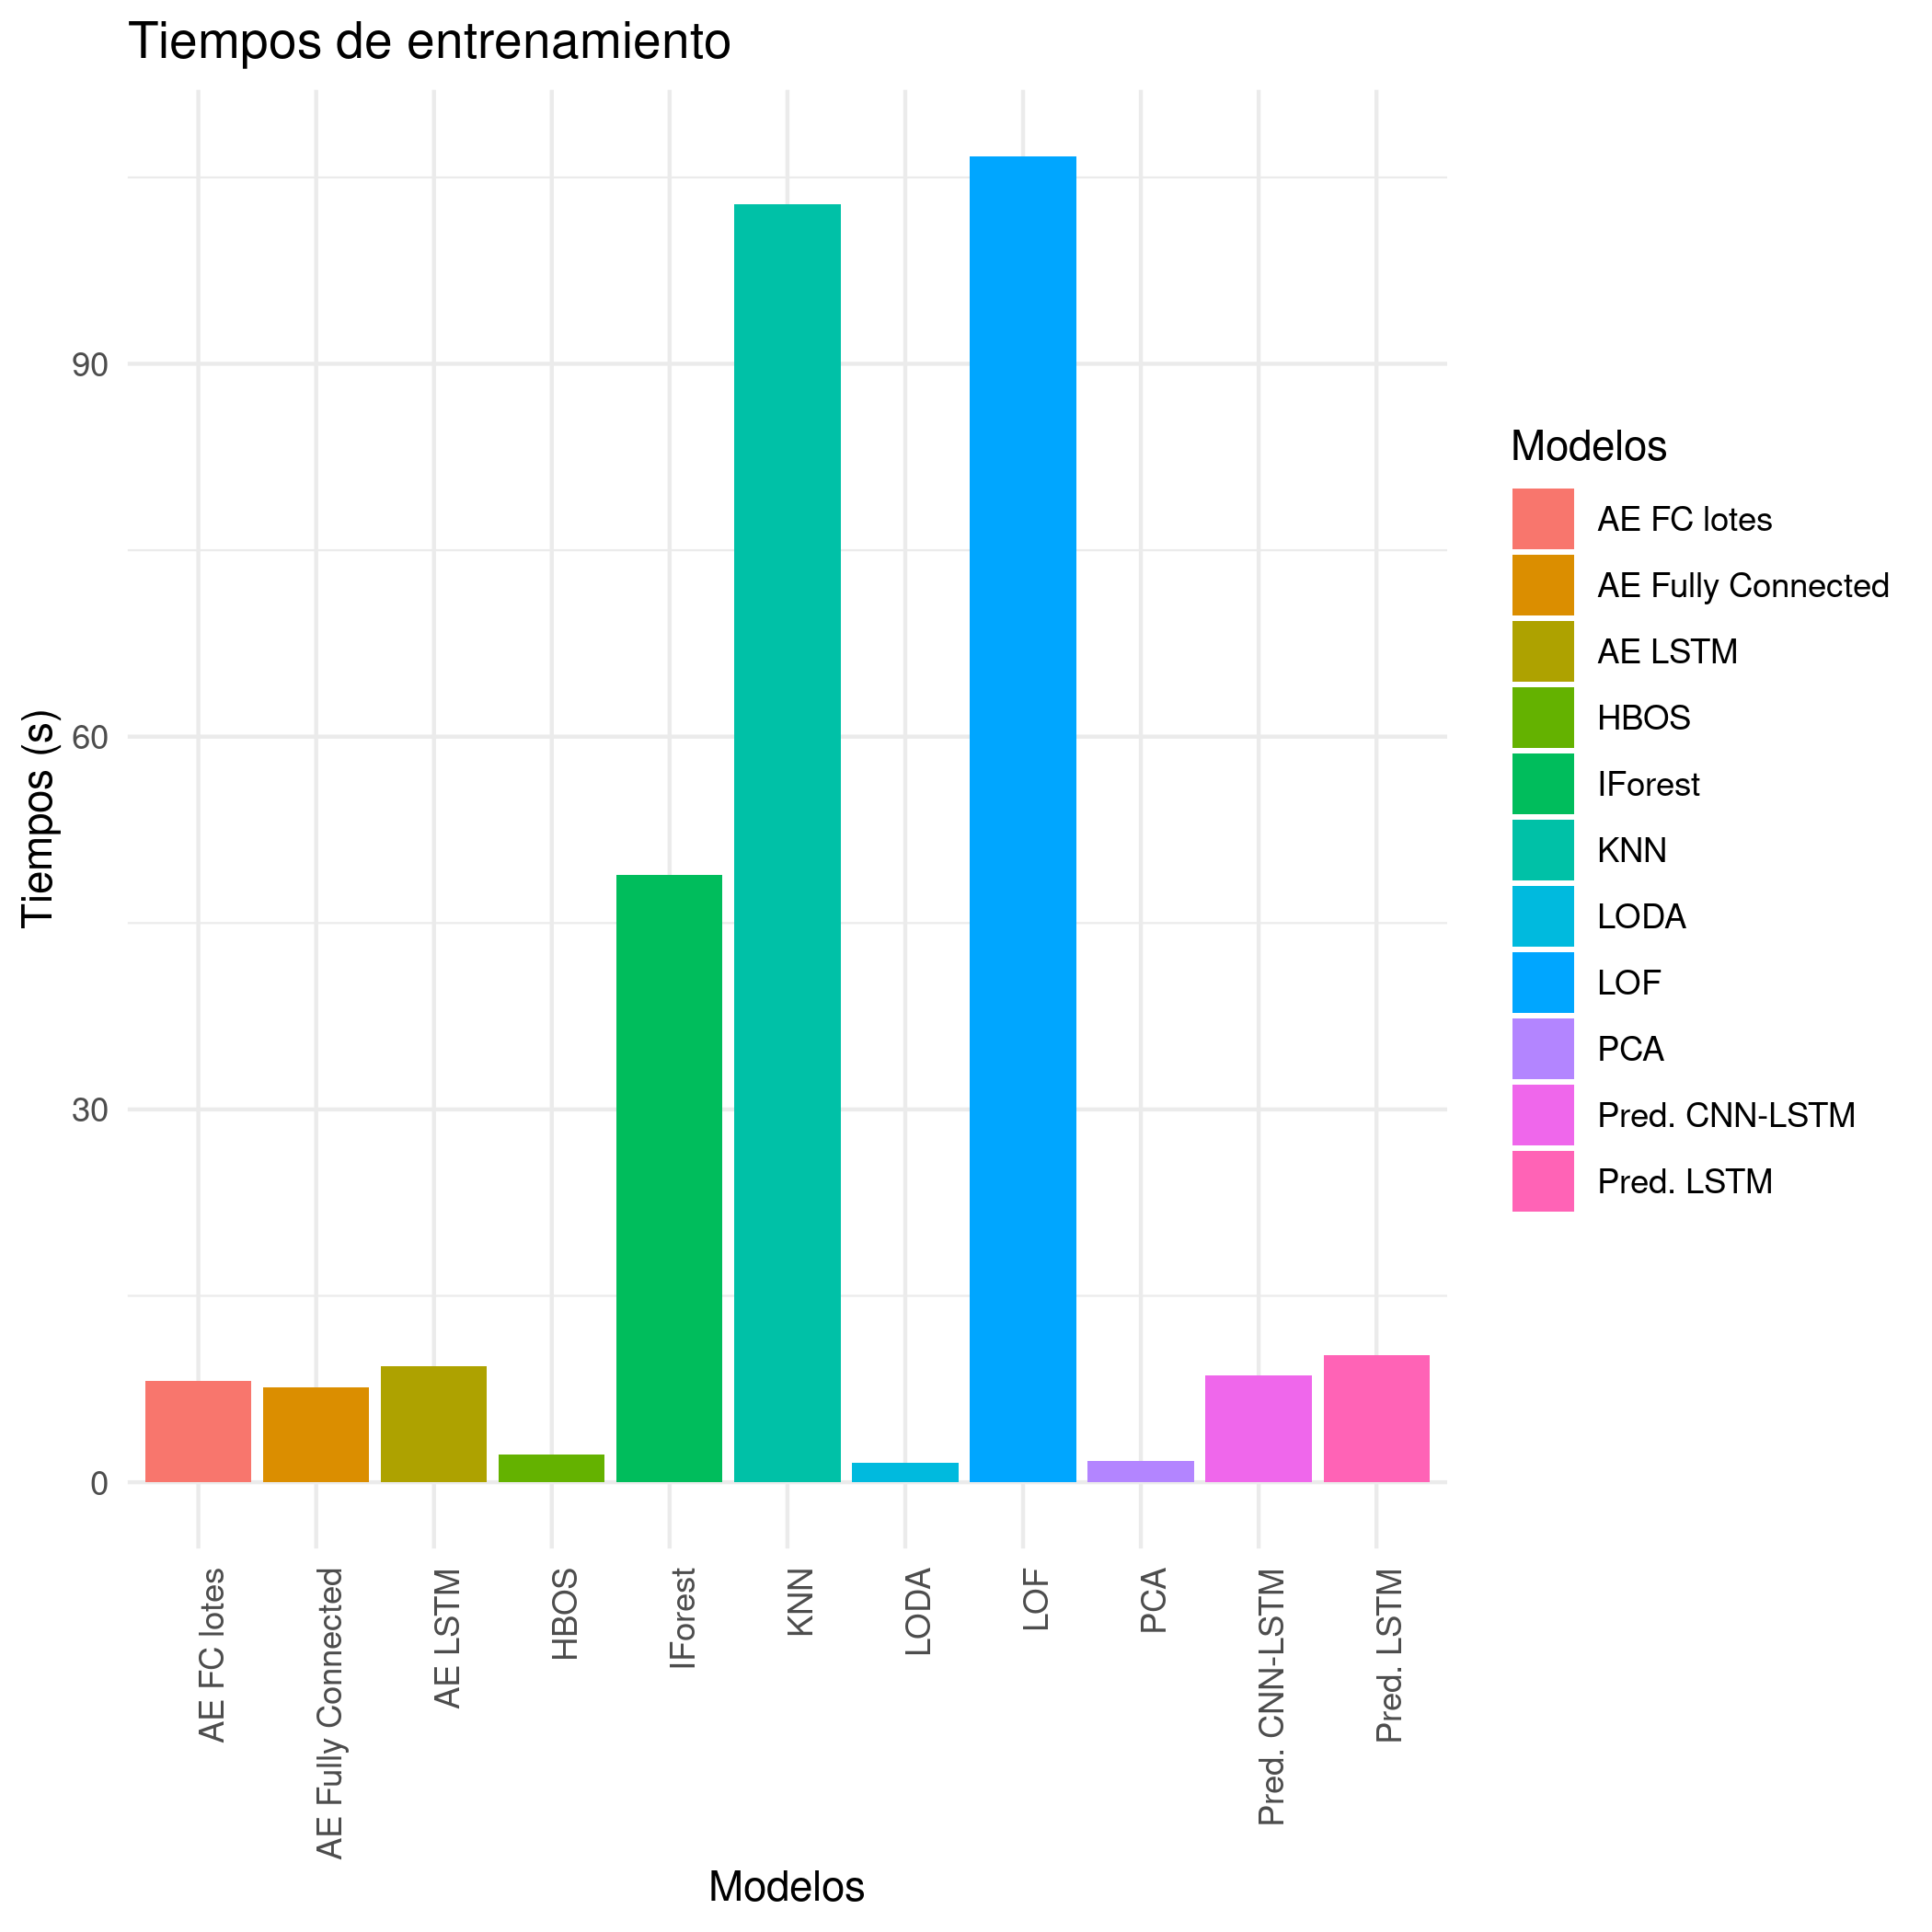
\includegraphics[scale=0.65]{imagenes/tiempos_prediccion2.png}
	\caption{Tiempos de predicción de los modelos sin Feature Bagging LOF.}
	\label{img:tiempos-prediccion2}
\end{figure}

Aquí podemos ver algo mejor los tiempos que consumen los algoritmos en predecir. Podemos ver que LOF y KNN son los que maś tiempo consumen en predecir, por encima de 90 segundos. Por otro lado tenemos Isolation Forest después de estos con alrededor de 40-45 segundos. Tras esto vienen el resto de modelos con unos tiempos mucho más bajos, todos con 10 segundos o menos en predecir un día de datos completo. 

Cabe decir que, por tiempo consumido, todos los modelos son viables en el uso para esta tarea, pero podemos ver claramente que los modelos Deep Learning consumen muy poco tiempo y en concreto, el modelo de predicción CNN-LSTM consume poco tiempo y es el modelo que mejor resultado nos ha arrojado.

Sobre estas comparativas de tiempos cabe resaltar las máquinas empleadas para los cálculos. Para todos los modelos se ha empleado la misma máquina aunque no siempre el mismo hardware. En el cómputo de los scores de anomalías y en los entrenamientos de los modelos que lo necesiten se ha empleado una máquina DGX-1. Esta máquina dispone de 8 tarjetas gráficas NVIDIA Tesla V100 con 32 GB de memoria, 5120 CUDA cores y 640 Tensor Cores. Posee 512 GB de memoria RAM y 80 núcleos aportados por dos procesadores Intel Xeon E5-2698.

Para el entrenamiento de los modelos Deep Learning se ha empleado una sola tarjeta gráfica al igual que para la predicción de los mismos modelos. Por otro lado, los modelos clásicos que tienen disponible paralelismo se han ejecutado sobre los 80 núcleos de la máquina para aprovechar el potencial al máximo.